\documentclass[11pt]{article}
\usepackage[utf8]{inputenc}
\usepackage[T1]{fontenc}
\usepackage{lmodern}
\usepackage[margin=1.05in]{geometry}
\usepackage{amsmath,amssymb,amsthm,mathtools}
\usepackage{enumitem}
\usepackage{booktabs}
\usepackage{graphicx}
\usepackage{xcolor}
\usepackage[colorlinks=true,linkcolor=blue!50!black,citecolor=green!40!black,urlcolor=blue!60!black]{hyperref}
\usepackage[capitalise,noabbrev]{cleveref}
\usepackage{algorithm}
\usepackage[noend]{algpseudocode}

\newtheorem{theorem}{Theorem}[section]
\newtheorem{lemma}[theorem]{Lemma}
\newtheorem{proposition}[theorem]{Proposition}
\newtheorem{corollary}[theorem]{Corollary}
\newtheorem{claim}[theorem]{Claim}
\theoremstyle{definition}
\newtheorem{definition}[theorem]{Definition}
\newtheorem{example}[theorem]{Example}
\newtheorem{remark}[theorem]{Remark}
\newtheorem{question}[theorem]{Open question}

\newcommand{\E}{\mathbb{E}}
\newcommand{\Prob}{\Pr}
\newcommand{\R}{\mathbb{R}}
\newcommand{\N}{\mathbb{N}}
\newcommand{\F}{\mathbb{F}}
\newcommand{\bits}{\{0,1\}}
\newcommand{\eps}{\varepsilon}
\newcommand{\poly}{\mathrm{poly}}
\newcommand{\polylog}{\mathrm{polylog}}
\newcommand{\supp}{\mathrm{supp}}
\newcommand{\sv}{\mathrm{var}}
\newcommand{\KL}{\mathrm{KL}}
\newcommand{\MC}{\mathrm{MC}}
\newcommand{\cost}{\mathrm{cost}}
\newcommand{\one}{\mathbf{1}}
\newcommand{\Lit}{\textsc{lit}}
\newcommand{\Sum}{\textsc{sum}}
\newcommand{\Prod}{\textsc{prod}}
\newcommand{\BoxL}{\textsc{box}}
\newcommand{\NP}{\mathsf{NP}}
\newcommand{\coNP}{\mathsf{coNP}}
\newcommand{\MA}{\mathsf{MA}}
\newcommand{\AM}{\mathsf{AM}}
\newcommand{\IP}{\mathsf{IP}}
\newcommand{\BPP}{\mathsf{BPP}}
\newcommand{\SBP}{\mathsf{SBP}}
\newcommand{\PH}{\mathsf{PH}}
\newcommand{\Ptime}{\mathsf{P}}


\title{Beating Monte Carlo on rare circuit outputs:\\ envelopes, proof-carrying sampling, and their limits}
\author{Claude (Anthropic), prompted by Kaarel H\"anni\\[2pt]
\small Research note, October 2026. Draft; proofs checked by AI referees, not by humans.}
\date{}

\begin{document}
\maketitle

\begin{abstract}
Given a Boolean circuit $C$ and a product distribution $D$, how can one estimate a
tiny $p=\Pr_D[C(x)=1]$ faster than Monte Carlo (cost $\approx1/p$) without ever
being wrong? We seek procedures sound on every circuit and efficient on wide classes,
alone or with one argument from an unbounded prover. Upper bounds need deduction,
lower bounds need proposals, and sampling pays for the surprise that is left: an
\emph{envelope}, a tractable $\varphi\ge\one_C$ with computable mass, turns a
deduction into an importance sampler whose cost is the looseness $K=\E_D\varphi/p$.
Without a prover, a Decompose--Force--Sample--Branch procedure is sound everywhere and
costs $\poly\cdot K$ when its ideal explanation tree is polynomial: read-once formulas,
read-once compositions of sub-circuits component-dense in their polarity, backdoor
triggers, small cutsets; envelope leaves and a meta-procedure add DNFs and DNNFs.
Circuits whose $\wedge$-gates are bracketed with logarithmic \emph{context width} have
polynomial-size DNNFs, hence FPRASs (e.g.\ ORs of bounded-pathwidth CNFs,
$\#\mathsf P$-hard to count). Further modules certify the presumption of independence,
make annealing sound, tilt thresholds of overlapping local
sub-circuits, and factor out affine structure; yet on random parity checks
decomposable envelopes with small leaves cost at least the square root of Monte
Carlo's price. With a prover, proof-carrying importance sampling over any
Cook--Reckhow proof system is sound against every argument and complete when the
rarity has a short proof of confinement to a tractable region, at cost
$\poly(|\pi|)+2^{\sigma_u}$ for deductive content of size $|\pi|$ and unexplained
surprise $\sigma_u$. Limits: no procedure beats sampling on all circuits unless
$\NP\subseteq\BPP$; no argument system is complete for upper bounds unless
$\coNP\subseteq\MA$; the prover strictly helps for upper bounds whenever slices of its
proof system's canonical pair are not separable in randomized polynomial time (e.g.\
for Frege, if Blum integers cannot be factored by polynomial-size circuits); and such
separations cannot rest on $\NP$-hardness via randomized many-one reductions with gap
at least $1+1/\poly$.
\end{abstract}

\tableofcontents

\section{Introduction}\label{sec:intro}

Let $C:\bits^n\to\bits$ be a Boolean circuit and $D$ a distribution on its inputs.
We want $p=\Pr_{x\sim D}[C(x)=1]$ when $p$ is tiny. Monte Carlo sampling finds
it to relative error $\eps$ with $\Theta(\log(1/\delta)/(p\eps^2))$ evaluations
of $C$: polynomial in $1/p$, so exponential in the \emph{surprise}
$\log_2(1/p)$ of the event. This note asks two questions.
\begin{enumerate}
\item \emph{Without help.} For which circuits can a polynomial-time procedure,
one that may check some property of the circuit and then sample, estimate $p$
to relative error at a cost polynomial in $\log(1/p)$ instead of $1/p$, while
never being wrong (beyond probability $\delta$) on any circuit?
\item \emph{With a prover.} An unbounded prover sends one argument; a
polynomial-time verifier checks it and samples. No argument may make the
verifier accept a false claim with probability above $\delta$, on any circuit.
For which circuits do convincing arguments exist?
\end{enumerate}
These are certified versions of the low-probability estimation problems studied
by the Alignment Research Center \cite{wu2024lowprob,christiano2022presumption},
where the aim is to estimate the probability of a rare behaviour of a model
faster than by sampling, using the model's internals.

\subsection{The picture}

One idea organises almost everything: \textbf{upper bounds need deduction;
lower bounds need proposals; sampling pays for whatever surprise is left}.
\begin{itemize}
\item A lower bound $p\ge L$ can be certified by exhibiting mass: a proposal
distribution concentrated where $C=1$, with computable likelihood ratios.
Clipped importance weights make this sound for any proposal (\cref{prop:proposal}).
\item An upper bound below the sampling scale cannot be certified by
evaluating $C$, however cleverly: a verifier that makes $T$ evaluations cannot
certify $p<1/T$ (up to constants), whatever argument it is given
(\cref{thm:blackbox,thm:surprise}). It must read the circuit and \emph{deduce}
that $C(x)=1$ confines $x$ to a region of small, exactly computable measure.
\item Combining the two, an \emph{envelope}, a tractable function $\varphi$ with
$\varphi\ge\one_C$ whose mass $Z=\E_D\varphi$ is computable and from which one can
sample, yields an importance sampler with bounded weights, hence two-sided
intervals, at cost $O(K\eps^{-2}\log(1/\delta))$ where $K=Z/p$
(\cref{thm:envelope}). The envelope explains $\log_2(1/Z)$ bits of the
surprise; the remaining $\log_2K$ bits are paid for by sampling, and this
residual cost is unavoidable for anything that treats the unexplained part as
a black box (\cref{thm:surprise}).
\end{itemize}
Karp--Luby--Madras estimation of DNF probabilities \cite{klm1989}, exact
counting for decision-DNNFs and bounded treewidth, exponential tilting for
large deviations \cite{siegmund1976} and the Chernoff bound are all instances.

\subsection{Results}

\paragraph{Limits (\cref{sec:limits}).} Beating sampling on all circuits is
impossible: it would put $\NP$ in $\BPP$, and with exponentially hard
pseudorandom generators no procedure beats sampling by more than a $p^{-o(1)}$
factor even on explicit small circuits (\cref{prop:worstcase}). With a prover, no
argument system is complete for upper bounds unless $\coNP\subseteq\MA$
(\cref{thm:ma}), and black-box verification of upper bounds is impossible
(\cref{thm:blackbox}). Interaction would trivialise the problem (sum-check
gives exact $p$ for every circuit), so the one-message model is the
interesting one.

\paragraph{Without a prover (\cref{sec:part1}).} The procedure DFSB
(Decompose--Force--Sample--Branch) recursively splits the event by exact rules
(independence of variable-disjoint parts, literals forced by propagation,
Shannon expansion) and samples only at leaves that are dense or have tight
envelopes. It is sound on every circuit, and complete, with cost
$O(m\,K\,d^2\eps^{-2}\log(m/\delta))$ evaluations, on every circuit whose ideal
$K$-explanation tree has $m$ nodes (\cref{thm:dfsb}). This covers products and
read-once compositions of arbitrary dense sub-circuits, backdoor-style triggers,
circuits with small cutsets (exactly, by cutset conditioning), DNFs and DNNFs, and,
through sound local rewriting, disguised versions of all of these. Specialised
modules add bounded treewidth (exact), thresholds of independent blocks (exponential
tilting with $K=O(\sqrt k)$, \cref{prop:tilting}), unate CNFs with sparse overlaps (a
deterministic Harris--Janson sandwich, \cref{thm:janson}, which certifies the
``presumption of independence''), and the known FPRAS classes
\cite{meel2026dnnf,moitra2019,gopalan2011fptas}.

\paragraph{With a prover (\cref{sec:part2}).} Proof-carrying importance sampling:
the argument is a DAG of deductive steps checked by any Cook--Reckhow proof
system (implications, exclusivity, independence) and sampling steps with
declared confidence budgets. It is sound on every circuit and every argument
(\cref{thm:pcis-sound}), and complete on every circuit that has a short proof of
being confined to a tractable region in which it is not rare
(\cref{thm:certenv}). Lower bounds need no proof at all. The verifier's cost is
$\poly(|\pi|)+2^{\sigma_u}$, where $\sigma_u$ is the surprise left unexplained by
the argument, and both terms are necessary in the black-box sense: each bit of
argument buys at most one bit of surprise (\cref{thm:surprise}). The prover helps
strictly: for lower bounds unless $\NP\subseteq\BPP$; for upper bounds exactly to
the extent that the verifier's proof system is not weakly automatable
(\cref{cor:automatability}); two-sidedly under the hardness of factoring. Such
separations cannot be based on $\NP$-hardness alone unless $\coNP\subseteq\AM$.

\paragraph{Experiments (\cref{sec:experiments}).} A Python implementation
(\texttt{rareprob}) estimates, e.g., $p\approx4\cdot10^{-44}$ for a threshold of 400
independent random blocks to $5\%$ with $5\cdot10^5$ samples, $p\approx7\cdot10^{-25}$
for an 80-bit trigger with $2\cdot10^4$ samples, and certifies a
$2^{-20}$-rare SPN-hidden trigger with a SAT-solver proof where all syntactic methods
fail; in 2{,}450 adversarial and random trials no interval missed $p$ more often
than allowed.

\subsection{Related work}

\emph{Approximate counting.} Karp--Luby--Madras \cite{klm1989} and the stopping
rule of \cite{dklr2000} are the prototypes; for self-reducible classes, approximate
counting and approximate sampling are equivalent \cite{jvv1986}, and Karger's
unreliability FPRAS \cite{karger1999} is an early instance of a combinatorial
theorem (few near-minimum cuts) serving as the envelope. FPRASs exist for DNNF
\cite{meel2026dnnf} (and before it nFBDD \cite{meel2025nfbdd} and NFA
\cite{arenas2021nfa}), for CNFs in the local-lemma regime
\cite{moitra2019,fgyz2021,fhy2021,jpv2021,hwy2022,wangyin2024}, and for knapsack
\cite{gopalan2011fptas,gkm2010}; d-DNNF, OBDD, SDD and bounded treewidth admit exact
counting \cite{darwiche2002map,samer2010}. Hashing-based counters
\cite{chakraborty2013approxmc} use an NP oracle; partial compilation with
sampling \cite{lai2023partialkc} and AND/OR importance sampling
\cite{gogate2008andor} combine decomposition with sampling for variance reduction,
without relative-error guarantees for rare events. Certified exact model counting
\cite{bryant2023cpog} checks compilation by proofs.
\emph{Rare-event simulation} \cite{asmussenglynn2007,bucklew2004} studies
importance sampling with bounded relative error; the soundness requirement
here (valid intervals on every input) is the computer-science twist.
\emph{Interactive proofs} certify exact counts \cite{lfkn1992} and lower bounds
\cite{gs1986}; the Merlin--Arthur setting connects to proof complexity
\cite{cookreckhow1979,kp1998,bpr2000,pudlak2003pairs} and to the class $\SBP$
\cite{bgm2006}.
\emph{Heuristic arguments.} ARC's programme
\cite{christiano2022presumption,hilton2024surprise,wu2024lowprob} seeks estimators
that use a model's internals to beat sampling, judged by ``surprise accounting'';
this note isolates the part of that programme that can be made sound, and shows
where soundness forces deduction. ARC's ``matching sampling principle''
\cite{neyman2025competing} asks for estimators that do at least as well as sampling
(on average over a distribution of circuits, without soundness), and its
``computational no-coincidence principle'' \cite{neyman2025nocoincidence}
conjectures that structure in random reversible circuits always has short
explanations checkable by a verifier; our Part~2 is a worst-case, statistically
sound relative of the latter, for probabilities instead of properties.

\section{Setting}\label{sec:setting}

\paragraph{Circuits.}
A circuit $C$ on inputs $x_1,\dots,x_n$ is a directed acyclic graph whose
leaves are the inputs and the constants $0$ and $1$, and whose internal nodes
(gates) compute $\wedge$, $\vee$ (any fan-in), $\neg$, $\oplus$ or a threshold
function $[\sum_j w_j y_j \ge t]$ of their inputs; one gate is the output. The
weights $w_j$ and the threshold $t$ are rationals given in binary (a
floating-point number stands for its exact binary value), and the comparison is
exact, with no tolerance (our implementation evaluates threshold gates the same
way). $|C|$ is the number of wires. For a gate $g$,
$\sv(g)\subseteq[n]$ is the set of input variables in its cone (its
\emph{support}; always the syntactic one). Pushing negations to the inputs gives
the negation normal form (NNF) of $C$: an $\{\wedge,\vee\}$-circuit over literals
and constants. For $\{\wedge,\vee,\neg\}$-circuits it has at most two copies of
every gate, one per polarity; a $\oplus$-gate of fan-in $k$ expands to $O(k)$ gates
per polarity, a threshold gate whose weights, scaled to integers, have polynomially
bounded total $W=\sum_j|w_j|$ expands by a sequential counter with $O(kW)$ wires (a
negative weight acts on the complemented input), and other gates stay opaque. An
$\wedge$-gate of an NNF is \emph{decomposable} if its children have pairwise
disjoint supports, and an $\vee$-gate is \emph{deterministic} if its children are
pairwise inconsistent; an NNF all of whose $\wedge$-gates are decomposable is a
DNNF, and a d-DNNF if moreover all its $\vee$-gates are deterministic
\cite{darwiche2002map}.

\paragraph{Distributions.}
$D$ is a product distribution on $\bits^n$ with rational marginals
$\Pr[x_i=1]=q_i$, again given in binary (a floating-point marginal stands for its
exact value). The \emph{input size} of $(C,D)$ is $|C|$ plus the total bit length
of the $q_i$ and of the weights and thresholds of $C$; running times that mention
only $|C|$ count arithmetic operations on such numbers. Product
structure is what makes ``disjoint supports'' mean ``independent''. A
distribution given by a sampler circuit $S:\bits^m\to\bits^n$ reduces to the
uniform case: $\Pr_{x\sim S(U_m)}[C(x)=1]=\Pr_{u\sim U_m}[(C\circ S)(u)=1]$.
(The reduction can destroy structure; we do not rely on it.) We write
\[
  p \;=\; p_D(C) \;=\; \Pr_{x\sim D}[C(x)=1]
\]
and think of $p$ as tiny: $2^{-50}$, $n^{-\omega(1)}$, or $2^{-\Omega(n)}$.
For a set or function $E$ we write $D(E)=\E_D[E]$.

\paragraph{What counts as an answer.}
Because $p$ can be arbitrarily small, additive error is useless; we ask for
relative error. To let a procedure decline, we let it output intervals.

\begin{definition}[sound interval estimation]\label{def:sound}
An \emph{estimation procedure} gets $(C,D,\eps,\delta)$ and outputs an
interval $[L,U]\subseteq[0,1]$ (possibly the trivial $[0,1]$, meaning ``no
verdict''). It is \emph{sound} if for every circuit $C$ and every $D$,
\[
\Pr\big[p_D(C)\notin[L,U]\big]\le\delta .
\]
It is \emph{complete} on a class $\mathcal C$ if for all $C\in\mathcal C$,
with probability at least $1-\delta$ the interval is tight:
$U\le(1+\eps)L$. It is \emph{efficient} if it runs in time polynomial in the
input size, $1/\eps$ and $\log(1/\delta)$.
\end{definition}

A sound procedure that is complete on $\mathcal C$ gives, on $\mathcal C$, a
$(1\pm\eps)$-approximation of $p$ with probability $1-2\delta$; outside
$\mathcal C$ its output is still a valid (if loose) interval. Soundness
everywhere is what makes the ``check a property, then sample'' procedures of
the problem statement safe to use on circuits we know nothing about.

\paragraph{The baseline.}
Monte Carlo draws $x^{(1)},\dots,x^{(N)}\sim D$ and reports the fraction of
ones. A relative-error interval needs
$N=\Theta\big(\log(1/\delta)/(p\eps^2)\big)$ samples, so its cost is
\[
\cost_{\MC}=\Theta\Big(\frac{|C|\log(1/\delta)}{p\,\eps^2}\Big),
\]
exponential in the \emph{surprise} $\log_2(1/p)$. The
Dagum--Karp--Luby--Ross stopping rule achieves this without knowing $p$ in
advance, and their algorithm $\mathcal{AA}$ is optimal up to a constant factor
among procedures that only see i.i.d.\ samples of a $[0,1]$-valued variable
\cite{dklr2000} (see \cite{chen2007inverse} for a repaired proof of the stopping-rule
guarantee); for $0/1$ samples of mean $p\ll1$ the optimal cost is
$\Theta(\log(1/\delta)/(p\eps^2))$. Beating sampling therefore requires looking at
the circuit.

\begin{definition}[beating sampling]
A procedure beats sampling on a class $\mathcal C$ if it is sound, efficient,
and complete on $\mathcal C$, and $\mathcal C$ contains circuits with
$p=n^{-\omega(1)}$ (for most of our classes, $p=2^{-\Omega(n)}$). Its cost is then
polynomial in the input size whatever $p$ is, whereas that of Monte Carlo grows like
$1/p$, exponentially in the surprise.
\end{definition}

\paragraph{Prover-assisted estimation.}
In the second setting an unbounded prover sends one string $\pi$ (an
\emph{argument}) to a randomized polynomial-time verifier $V$, which then
flips coins (for instance to sample) and outputs an interval $[L,U]$.

\begin{definition}[argument system]\label{def:argument}
$V$ is \emph{sound} if for every circuit $C$, every $D$ and every string
$\pi$, $\Pr_{\text{coins of }V}\big[p_D(C)\notin V(C,D,\pi,\eps,\delta)\big]\le\delta$.
It is \emph{complete} on $\mathcal C$ if for every $C\in\mathcal C$ there is a
$\pi$ of size polynomial in the input size such that with probability $1-\delta$
the output is tight. One-sided variants (lower-bound or upper-bound arguments) are defined
in the obvious way.
\end{definition}

This is the non-interactive, statistically sound (Merlin--Arthur) model. We
will see in \cref{sec:limits} that interaction (or computational soundness in the
random-oracle model) would trivialise the problem, while in this model upper bounds on $p$ cannot be
certified for all circuits unless $\coNP\subseteq\MA$.

\section{Limits}\label{sec:limits}

This section fixes what cannot be done, so that the positive results of
\cref{sec:envelopes,sec:part1,sec:part2} can be read against it.

\subsection{Without a prover: structure is necessary}

\begin{proposition}[worst case]\label{prop:worstcase}
\begin{enumerate}[label=(\alph*)]
\item If a sound efficient procedure is complete (for any fixed $\eps<1$) on
all 3-CNF formulas under the uniform distribution, then $\NP\subseteq\BPP$.
\item Let $G_k:\bits^k\to\bits^{2k}$ be computable by $\poly(k)$-size
circuits and suppose every circuit of size $T(k)$ distinguishes $G_k(U_k)$
from $U_{2k}$ with advantage less than $1/2$. For $y\in\bits^{2k}$ let
$C_y(x)=[G_k(x)=y]$ on inputs $x\in\bits^k$. Then $p(C_{G(s)})\ge 2^{-k}$ for
every seed $s$, while $\Pr_y[p(C_y)>0]\le2^{-k}$ for uniform $y$; and any
sound procedure with $\delta\le1/8$ that is complete on $\{C_{G(s)}\}$ runs in
time at least $T(k)-\poly(k)$ on some $C_{G(s)}$.
\end{enumerate}
\end{proposition}

\begin{proof}
(a) If $p=0$, a tight interval must be $[0,0]$; if $p>0$ (so $p\ge2^{-n}$) a
tight interval that contains $p$ has $L>0$. Answering ``satisfiable'' iff $L>0$
errs with probability at most $\delta$.
(b) The bounds on $p$ are immediate ($\E_y|G^{-1}(y)|=2^{k-2k}$). Let $A$ be
the procedure and $t$ its running time on the family. Consider the test
``$A(C_y)$ outputs $L>0$''. On $y=G(s)$ it fires with probability at least
$1-\delta$ (a tight interval around $p>0$ has $L>0$). On uniform $y$, with
probability at least $1-2^{-k}$ we have $p=0$ and soundness forces $L\le
p=0$ except with probability $\delta$. The advantage is at least
$1-2\delta-2^{-k}>1/2$; fixing $A$'s coins to their best value gives a circuit
of size $t+\poly(k)$, so $t\ge T(k)-\poly(k)$.
\end{proof}

Monte Carlo on $C_{G(s)}$ costs $O(2^k\poly(k))$. So if $G$ is
exponentially hard ($T(k)=2^{(1-o(1))k}$), no sound procedure beats sampling on
this family by more than a $2^{o(k)}=p^{-o(1)}$ factor, even though every
instance is a small, explicit circuit. Beating sampling is a matter of
structure: the classes of \cref{sec:part1} are where the structure is visible to
a polynomial-time algorithm, and those of \cref{sec:part2} are where it is
visible to a polynomial-time verifier given a hint.

\subsection{With a prover: upper bounds need deduction}

Lower and upper bounds behave very differently. A lower bound $p\ge L$ can be
witnessed by \emph{showing} probability mass: a proposal distribution $Q$
concentrated on $C^{-1}(1)$ (\cref{sec:lower}). An upper bound must exclude
mass that the verifier has not seen. The next theorem makes this precise:
a verifier that only evaluates $C$ cannot certify an upper bound much below
the reciprocal of its number of evaluations, whatever argument it is given.

\begin{theorem}[sampling cannot certify upper bounds]\label{thm:blackbox}
Let $V$ be a verifier that receives an argument $\pi$, has oracle access to
$f:\bits^n\to\bits$, flips coins, makes at most $T$ oracle queries (at
adaptively chosen points, from any distributions it likes), and outputs a
number $U$. Suppose $V$ is sound for upper bounds under the uniform
distribution: for all $f,\pi$, $\Pr[U<p(f)]\le\delta$. Then for every $f$,
every $\pi$ and every $k\le n$,
\[
\Pr\big[V^f(\pi)\text{ outputs }U<2^{-k}\big]\;\le\;\delta+T\,2^{-k}.
\]
In particular, to output an upper bound below $\eta$ with probability
$1-\delta'$ a black-box verifier needs $T\ge(1-\delta-\delta')/(2\eta)$
queries.
\end{theorem}

\begin{proof}
Fix $f$, $\pi$, $k$. For $t\in\bits^k$ let $H_t=\{x:x_{1..k}=t\}$ and
$f_t=f\vee\one_{H_t}$, so $p(f_t)\ge2^{-k}$. Fix the coins $r$ of $V$. The run
of $V^f(\pi;r)$ queries a fixed sequence of points $z_1,\dots,z_T$. The run of
$V^{f_t}(\pi;r)$ is identical unless some $z_i\in H_t$; for each fixed $z_i$
this happens for exactly one $t$. Hence for uniform $t$,
$\Pr_{r,t}[\text{the runs differ}]\le T2^{-k}$, and
\[
\E_t\Pr_r\big[V^{f_t}(\pi;r)<2^{-k}\big]\;\ge\;\Pr_r\big[V^{f}(\pi;r)<2^{-k}\big]-T2^{-k}.
\]
Some $t$ attains at least the average; for it, $V$ outputs $U<2^{-k}\le
p(f_t)$ with that probability, which soundness bounds by $\delta$.
For the last claim take $k=\lceil\log_2(1/\eta)\rceil-1$, so that
$\eta\le 2^{-k}<2\eta$.
\end{proof}

\begin{remark}
The same argument works for any distribution $D$ with enough min-entropy,
planting $H=\{x:Ax=b\}$ for a random $k\times n$ matrix $A$ over $\F_2$ and
random $b$: every fixed point lies in $H$ with probability $2^{-k}$, and by
pairwise independence $D(H)\ge2^{-k-1}$ with probability $1-4\cdot2^{k}\sum_x
D(x)^2$. The planted circuit $f\vee[Ax=b]$ is only $O(nk)$ gates larger, so
the theorem also holds for white-box verifiers that look at $C$ only through
evaluations and its size.
\end{remark}

The verifiers of \cref{sec:part2} escape \cref{thm:blackbox} by reading the
circuit: they check a proof that $C(x)=1$ forces $x$ into a region of small,
exactly computable measure. In general such proofs cannot always exist:

\begin{theorem}[no complete upper-bound arguments]\label{thm:ma}
Suppose a sound argument system (soundness error $\delta\le1/3$) is complete
for upper bounds on all 3-CNF formulas with $p=0$ under the uniform
distribution, i.e.\ for each such $C$ some $\pi$ of polynomial size makes $V$
output $U<2^{-n}$ with probability at least $2/3$. Then $\coNP\subseteq\MA$,
and the polynomial hierarchy collapses to its second level.
\end{theorem}

\begin{proof}
Merlin sends $\pi$; Arthur runs $V$ and accepts iff $U<2^{-n}$. If $C$ is
unsatisfiable he accepts with probability $\ge2/3$. If $C$ is satisfiable then
$p\ge2^{-n}$, and accepting means $V$ output $U<p$, which happens with
probability at most $1/3$. So 3-UNSAT$\in\MA\subseteq\AM$, and
$\coNP\subseteq\AM$ collapses $\PH$ to $\Sigma_2^p$ \cite{bhz1987}.
\end{proof}

The lower-bound side is weaker but not free: a system complete for lower
bounds within a constant factor on all circuits is exactly a proof that the
class $\SBP$ of \cite{bgm2006} is contained in $\MA$; since
$\MA\subseteq\SBP\subseteq\AM$ and the inclusions are not known to collapse,
we should not expect proposal-based lower bounds for every circuit either.

\subsection{Interaction trivialises the problem}

The restriction to one message is essential:

\begin{proposition}\label{prop:interactive}
\begin{enumerate}[label=(\alph*)]
\item (Sum-check \cite{lfkn1992}.) For every circuit $C$ and product $D$ with
dyadic marginals, the exact value of $p$ has an interactive proof with a
polynomial-time verifier, $O(n+|C|)$ rounds and soundness error
$O((n+|C|)\,d/|\F|)$, where $d$ bounds the individual degrees of the
arithmetised Tseitin constraint polynomial.
\item (Set lower bounds \cite{gs1986}.) Two-round public-coin protocols certify
$p\ge L$ within a constant factor for every circuit.
\end{enumerate}
\end{proposition}

Applying the Fiat--Shamir transform to (a) gives a one-message argument that
is only computationally sound, which is not the model asked for. So the
interesting question is the Merlin--Arthur one, where by
\cref{thm:blackbox,thm:ma} an argument must contain \emph{deductive} content
about the circuit, and can be complete only on a restricted class.

\section{Envelopes: the common mechanism}\label{sec:envelopes}

Most of our upper-bound-capable methods, with and without a prover, are
instances of one estimator (the exceptions are the correlation-inequality bounds
of \cref{sec:janson,sec:independence}, the product-of-ratios estimators of
\cref{sec:cftp}, and two variants of it: the counter-guided sampler of
\cref{thm:sis}, and the tilted Gibbs estimator of \cref{sec:local}, whose mass and
proposal are themselves certified statistically). It turns a \emph{deductive}
fact (``$C(x)=1$ implies $\varphi(x)\ge1$'') and an \emph{exact} computation
($\E_D\varphi$) into an importance sampler whose cost depends only on how loose
the deduction is.

\subsection{Envelope circuits}

\begin{definition}[envelope]\label{def:envelope}
An \emph{envelope circuit} $\Phi$ is an arithmetic circuit whose leaves are
literal indicators $[x_i=b]$, nonnegative rational constants, and
(\cref{sec:boxes}) \emph{boxes} $[B(x)=1]$ for circuits $B$; whose gates are
$\Sum$ and $\Prod$; and whose $\Prod$ gates are \emph{decomposable}: their children
have pairwise disjoint supports, where the support $\sv(v)$ of a node is the set of
variables occurring at the leaves of its cone ($\sv(B)$ for a box). We also require
that every $\Prod$-child with empty support be a constant leaf (fold constant
subcircuits first). $\Phi$ computes $\varphi:\bits^n\to\R_{\ge0}$. It
\emph{dominates} $C$ if $\varphi(x)\ge1$ whenever $C(x)=1$. Its \emph{mass} is
$Z=\E_D\varphi$; if $p>0$, its \emph{looseness on $C$} is $K=Z/p$, and domination
gives $Z\ge p$, i.e.\ $K\ge1$.
\end{definition}

A \emph{derivation} of $\Phi$ is a proof tree of its tree unfolding: keep,
top-down, one child of every $\Sum$ occurrence and all children of every $\Prod$
occurrence. By decomposability a derivation visits each node of nonempty support
at most once. With literal leaves and unit constants, $\varphi(x)$ is the number of
derivations all of whose leaves are satisfied by $x$; with general constants it is
the corresponding weighted count. A DNF $\bigvee_j T_j$ with consistent,
duplicate-free terms gives the envelope $\sum_j\prod_{\ell\in T_j}[\ell]$, and a DNNF
gives the envelope obtained by reading $\vee$ as $\Sum$ and $\wedge$ as $\Prod$.

\begin{lemma}[exact mass, exact sampling]\label{lem:envmass}
Let $\Phi$ have literal and constant leaves only, $D$ be a product distribution
with rational marginals, and $Z>0$. Then $Z=\E_D\varphi$ is computed by one
bottom-up pass ($\Sum\mapsto$ sum of children's masses, $\Prod\mapsto$ product)
with $O(|\Phi|)$ operations on rationals of $\poly(|\Phi|,b)$ bits ($b$ the total
bit length of the marginals and of the constants of $\Phi$), and the following
top-down procedure samples exactly from $Q_\varphi(x)=D(x)\varphi(x)/Z$: at a
$\Sum$ gate choose a child with probability proportional to its mass; at a
$\Prod$ gate visit all children; at a literal leaf set the literal; finally draw
every unset variable from $D$.
\end{lemma}

\begin{proof}
By decomposability and independence, $\E_D\prod_c\varphi_c=\prod_c\E_D\varphi_c$;
linearity handles $\Sum$. The procedure selects a derivation $\mathcal T$ with
probability $w(\mathcal T)/Z$, where $w(\mathcal T)$ is the product of the
literals' probabilities and the constants in $\mathcal T$ (the choice probabilities
telescope), and then draws $x\sim D$ conditioned on all literals of $\mathcal T$,
whose density is $D(x)\one[x\models\mathcal T]\,c(\mathcal T)/w(\mathcal T)$ with
$c(\mathcal T)$ the product of its constants. Summing over derivations,
$\Pr[x]=\sum_{\mathcal T}c(\mathcal T)D(x)\one[x\models\mathcal T]/Z=D(x)\varphi(x)/Z$.
(A literal is set at most once per derivation: two literals on the same variable
in one derivation would lie below different children of a decomposable $\Prod$.)
Bit lengths: the mass of a node is a sum of at most $2^{|\Phi|}$ products of at most
$|\Phi|$ constants and marginals.
\end{proof}

In floating point, masses must be kept in the log domain and the final interval
widened by the accumulated rounding error. Our implementation does exactly this:
along every derivation the computed weight and the sampler's choice probabilities
telescope, so the relative error of $\hat Z\cdot\E_{\hat Q}W$ is at most
$e^{\pm\eta}$, where $\eta$ is the largest sum of local rounding errors on a
derivation (a max-sum dynamic program over $\Phi$); the discreteness of the
categorical draws at $\Sum$ gates adds an absolute $O((n+|\Phi|)2^{-53})$ to $\E W$
(the remaining inputs are drawn from $D$ exactly, by comparing lazily drawn binary
digits of a uniform with those of $q_i$, so the rejection fills of
\cref{sec:boxes} are exact and the box estimates rest on exact samples); and the
output interval is widened by both and rounded outwards.

\subsection{The envelope estimator}

For $N$ i.i.d.\ samples in $[0,1]$ with empirical mean $\hat\mu$, the
\emph{Hoeffding--KL interval} at level $\delta$ is
$\{m\in[0,1]:N\,\KL(\hat\mu\|m)\le\ln(2/\delta)\}$ with $\KL$ the Bernoulli relative
entropy; it contains the true mean with probability at least $1-\delta$
\cite[Thm.~1]{hoeffding1963}. (In floating point our implementation excludes a value
only when its computed divergence exceeds the bound by more than its rounding error,
and allows for the rounding of $\hat\mu$, so the computed interval contains the exact
one.)

\begin{theorem}[envelope estimator]\label{thm:envelope}
Let $\varphi:\bits^n\to\R_{\ge0}$ dominate $C$, with exact mass $Z$ and an exact
sampler for $Q_\varphi=D\varphi/Z$ (for instance an envelope circuit with
\cref{lem:envmass}). If $Z=0$, output $[0,0]$ (valid under domination). Otherwise,
for $X\sim Q_\varphi$ let $W=C(X)/\varphi(X)$. Then
\begin{enumerate}[label=(\roman*)]
\item $W\in[0,1]$ and $\E W=p/Z=1/K$;
\item from $N$ independent copies, the Hoeffding--KL interval $[\ell,u]$ for
$\E W$ at level $\delta$ gives an interval $[Z\ell,\min(Zu,1)]$ containing $p$ with
probability at least $1-\delta$, \emph{for every circuit $C$} as long as $\varphi$
dominates it;
\item if $\varphi$ does not dominate $C$: for integer-valued $\varphi$ (envelope
circuits with literal leaves and integer constants) the same procedure gives a
valid interval for $\Pr_D[C(x)=1\wedge\varphi(x)>0]\le p$; for general $\varphi$, with
$W$ clipped at $1$, $Z\ell$ is still a valid lower bound on $p$;
\item for $0<\eps\le1$, run sequentially from
$N_0=\lceil c\log(2/\delta_1)/\eps^2\rceil$ samples, doubling $N$ and using level
$\delta_j=6\delta/(\pi^2j^2)$ at stage $j$: all intervals are valid with probability
$1-\delta$, and if $p>0$ the procedure reaches $u\le(1+\eps)\ell$ after
$N=O\big(K(\log(1/\delta)+\log\log K)/\eps^2\big)$ samples with probability $1-\delta$
(so both hold with probability $1-2\delta$). With a sample cap it always halts,
returning its current, still valid, interval. Each sample costs $O(|C|+|\Phi|)$
arithmetic operations with the sampler of \cref{lem:envmass}.
\end{enumerate}
\end{theorem}

\begin{proof}
(i) If $Q_\varphi(x)>0$ then $\varphi(x)>0$; if moreover $C(x)=1$ then
$\varphi(x)\ge1$, so $W\le1$. $\E W=\sum_xD(x)\varphi(x)C(x)/(Z\varphi(x))=p/Z$.
(ii) The KL interval is valid for i.i.d.\ $[0,1]$ variables, and $p\le1$.
(iii) For integer-valued $\varphi$, $\varphi(x)>0$ implies $\varphi(x)\ge1$, so
$W\in[0,1]$ and $\E W=\Pr[C=1,\varphi>0]/Z$. For real-valued $\varphi$, clipping
only lowers the mean, so $\E\min(W,1)\le\Pr[C=1,\varphi>0]/Z\le p/Z$.
(iv) Let $\mu=1/K$. By the multiplicative Chernoff bound, once
$N\ge c\log(1/\delta_j)/(\mu\eps^2)$ the empirical mean $\hat\mu$ is within a factor
$1\pm\eps/8$ of $\mu$ with probability $1-\delta_j$. Since
$\KL(a\|b)\ge(a-b)^2/(2\max(a,b))$, every $m$ in the KL interval with $m>\hat\mu$
satisfies $(m-\hat\mu)^2\le am$ with $a=2\log(2/\delta_j)/N$, hence
$m-\hat\mu\le a+\sqrt{a\hat\mu}$, and similarly below; for a suitable constant $c$
both are at most $(\eps/4)\hat\mu$, so $u/\ell\le(1+\eps/4)/(1-\eps/4)\le1+\eps$. With
the stated $N_0$, the first stage at which this holds has $j=O(\log K)$, whence the
$\log\log K$ term; the union bound over stages makes all intervals simultaneously
valid.
\end{proof}

So the cost of an envelope is governed by one number. Monte Carlo is the
trivial envelope $\varphi\equiv1$, with $K=1/p$; exact computation is $\varphi=C$
(when $C$ is itself a d-DNNF), with $K=1$. In between:

\begin{lemma}[what $K$ measures]\label{lem:K}
For $p>0$, $K=\E_D[\varphi\mid C=1]+\E_D[\varphi\,\one_{C=0}]/p$. For an envelope
with literal leaves and unit constants whose positivity set $\{\varphi>0\}$ equals
$C^{-1}(1)$ (e.g.\ a DNNF for $C$), $K$ is the expected number of satisfied
derivations of $x\sim D\mid C=1$, its \emph{expected ambiguity}. For a DNF with
$m$ terms, $K\le m$.
\end{lemma}

The first term is overcounting (union bounds); the second is mass that the
deduction failed to exclude. $K$ also bounds the relative variance
$\rho=\frac{Z}{p}\E_D[1/\varphi\mid C=1]-1\le K-1$ of $ZW$. The KL procedure of
\cref{thm:envelope}(iv) ignores the variance and pays $\Theta(K)$ samples whatever
$\rho$ is; a variance-adaptive interval (empirical Bernstein, or DKLR's algorithm
$\mathcal{AA}$) pays $O\big((\rho/\eps^2+K/\eps)\log(1/\delta)\big)$, so a low dispersion
of the derivation count helps only in the $\eps^{-2}$ term. The $K/\eps$ term cannot
be avoided by a sound procedure that uses the weights as a black box, and for tilting
envelopes $K$ can exceed $\rho$ exponentially (\cref{prop:certgap}). A d-DNNF has
$\varphi=\one_C$, $K=1$ and $\rho=0$. For $E=\bigwedge_{i\le m}(x_i\vee y_i)$ under the uniform
distribution, used as its own envelope, $K=(4/3)^m$, and the relative variance is at
least $(10/9)^m-1$ under every reweighting of its $\vee$-edges (with equality for unit
weights); both are exponential although $D(E)=(3/4)^m$ is known exactly.
\Cref{thm:sis} removes this overcounting altogether: its looseness is $D(E)/p$ rather
than $\E_D[\varphi]/p$.

In the spirit of surprise accounting \cite{hilton2024surprise}: of the $\log_2(1/p)$
bits of surprise in the event $C(x)=1$, an envelope with $Z\le1$ explains
$\log_2(1/Z)$ bits by deduction and exact computation (once domination is certified,
syntactically or by a proof), and leaves $\log_2K$ bits to sampling, at a cost of
about $K$ samples (up to $\eps^{-2}\log(1/\delta)$ factors). If $Z\ge1$ the envelope is
worse than Monte Carlo and is replaced by $\varphi\equiv1$. Monte Carlo explains
nothing; exact computation explains everything, with $|\Phi|$ possibly exponential
in $|C|$. Surprise accounting also charges the explanation's own description length:
zero for envelopes computed from $C$, and $|\pi|$ for prover-supplied ones
(\cref{thm:surprise}).

\subsection{Dense leaves}\label{sec:boxes}

Products of independent events that are individually not rare are the most
common source of rarity, and they need not have small envelopes: an
$\wedge$ of $k$ independent random sub-circuits $B_j$, each true with
probability $1/2$, has $p=2^{-k}$ but its literal envelope may lose a constant
factor per block. Boxes repair this: a box is a sub-function used as its own
envelope, its mass estimated by Monte Carlo and its conditional distribution
sampled by rejection. Estimation errors in the masses bias the proposal, but
the bias on each derivation is a product of per-box ratios that we can bound
exactly.

\begin{theorem}[envelopes with dense leaves]\label{thm:boxes}
Let $\Phi$ dominate $C$, with literal leaves and box leaves $B_1,\dots,B_r$
($\Prod$ gates decomposable with respect to supports), where
$m_j=D(B_j)\ge1/R$ and every derivation contains at most $L$ box leaves; let
$0<\eps\le1$. Estimate each $m_j$ by Monte Carlo to an interval $[\ell_j,u_j]$ at
level $\delta/(2r)$ with point value $\hat m_j$; compute masses $\hat Z$ and sample
$\hat Q$ as in \cref{lem:envmass} with $\hat m_j$ in place of $m_j$, filling each box
by rejection sampling from $D$. For $\rho(\mathcal T)=\prod_{B_j\in\mathcal
T}\hat m_j/m_j$ let $\rho_{\min},\rho_{\max}$ be its extreme values over derivations
when each $m_j$ ranges over $[\ell_j,u_j]$ (computed by a min-/max-product pass over
$\Phi$). Then, with $[\ell,u]$ a valid KL interval for $\E_{\hat Q}W$, $W=C/\varphi$, at
total level $\delta/2$ (fixed or sequential),
\[
p\in\big[\hat Z\ell/\rho_{\max},\;\hat Zu/\rho_{\min}\big]
\]
with probability at least $1-\delta$. If each box interval satisfies
$u_j\le(1+\eps/(8L))\ell_j$ and importance sampling is run to ratio
$1+\eps/4$, the output is tight with probability $1-2\delta$, after
$O(K(\log(1/\delta)+\log\log K)/\eps^2)$ samples of $\hat Q$, each costing
$O(|C|+|\Phi|+\sum_j|B_j|+LR\max_j|B_j|)$ in expectation; estimating the boxes costs
$O(rL^2R\log(r/\delta)/\eps^2)$ evaluations.
\end{theorem}

\begin{proof}
The sampler picks derivation $\mathcal T$ with probability
$\hat w(\mathcal T)/\hat Z$ where $\hat w$ uses the $\hat m_j$, and then draws
$x$ exactly from $D$ conditioned on $\mathcal T$'s leaves (rejection sampling
is exact; decomposability makes the leaves' conditionings independent), whose
density is $D(x)\one[x\models\mathcal T]/w(\mathcal T)$ with the true masses.
Hence $\hat Q(x)=\frac{D(x)}{\hat Z}\sum_{\mathcal T\ni x}\rho(\mathcal T)$, and
\[
\hat Z\,\E_{\hat Q}W=\sum_xD(x)C(x)\cdot\frac{1}{\varphi(x)}\sum_{\mathcal
T\ni x}\rho(\mathcal T)\;\in\;[\rho_{\min},\rho_{\max}]\cdot p,
\]
because $\varphi(x)$ is the number of derivations satisfied by $x$, so the
middle factor is an average of $\rho(\mathcal T)$. On the event (probability
$\ge1-\delta/2$) that all $m_j\in[\ell_j,u_j]$, $\rho_{\min}$ and $\rho_{\max}$
bound this average; conditionally on the box estimates the KL interval fails
with probability at most $\delta/2$. For tightness: $\rho_{\max}/\rho_{\min}\le
(1+\eps/(8L))^{2L}\le e^{\eps/4}$ and $(1+\eps/4)e^{\eps/4}\le1+\eps$ for $\eps\le1$.
Since $\hat Z=\sum_{\mathcal T}\rho(\mathcal T)w(\mathcal T)\le\rho_{\max}Z$, the mean
of $W$ under $\hat Q$ is at least $\rho_{\min}p/(\rho_{\max}Z)\ge e^{-\eps/4}/K$, so
\cref{thm:envelope}(iv) (which only needs i.i.d.\ $[0,1]$ samples of that mean)
gives the sample count. Computing $\varphi(X)$ evaluates every box, hence the
$\sum_j|B_j|$ term.
\end{proof}

With boxes, a product of $k$ independent dense blocks has $K=1$ and costs
$O(k^3R\log(k/\delta)/\eps^2)$ evaluations, against $2^{\Theta(k)}$ for Monte
Carlo; a DNF whose terms are products of dense blocks has an envelope (a $\Sum$ of
$\Prod$s of boxes) whose positivity set is $C^{-1}(1)$ and with $\varphi\le m$, so
$K\le m$ by \cref{lem:K}.

\subsection{Soft envelopes: Chernoff bounds as certificates}\label{sec:tilting}

Envelopes need not be integer-valued. If
$C(x)=[S(x)\ge t]$ with $S=\sum_{j=1}^k g_j(x_{B_j})$ a sum of
$\{0,1\}$-valued sub-circuits on disjoint blocks (since $S$ is an integer and the
comparison is exact, we take $t$ to be an integer, replacing it by $\lceil t\rceil$),
then for $\theta\ge0$
\[
\varphi_\theta(x)=e^{-\theta t}\prod_{j=1}^k\big([g_j=0]+e^{\theta}[g_j=1]\big)=e^{\theta(S(x)-t)}\ \ge\ \one[S(x)\ge t],\quad
Z_\theta=e^{-\theta t}\prod_{j=1}^k\big(1-p_j+p_je^{\theta}\big),
\]
where $p_j=D(g_j=1)$. $Z_\theta$ is the Chernoff bound, a deductively valid
upper bound, and $Q_{\varphi_\theta}$ is the exponentially tilted product
distribution. To sample it block by block we assume that the $p_j$ are known
exactly and $D$ conditioned on $g_j=b$ can be sampled, e.g.\ blocks small enough
to enumerate (as in our implementation), or boxes with $\min(p_j,1-p_j)\ge1/R$, in
which case \cref{thm:boxes} applies with $L=k$ (with weighted averages of $\rho$).
This is the classical efficient importance sampler for large deviations of sums
\cite{siegmund1976,bucklew2004}; here is a clean uniform bound on its looseness.

\begin{proposition}[tilting is polynomially tight]\label{prop:tilting}
Let the weights be $1$, $\E_D S\le t<k_+$, where $k_+=|\{j:p_j>0\}|$ and $t$ is an
integer. There is $\theta\ge0$ with $\E_{Q_\theta}S=t$, and for it
$K=Z_\theta/p\le\tfrac43\big(2\sqrt{k}+1\big)$. The same bound holds for any
$\theta\ge0$ with $|\E_{Q_\theta}S-t|<1/(k+2)$, so $\theta$ may be found by bisection
and $e^\theta$ taken rational.
\end{proposition}

\begin{proof}
$\theta\mapsto\E_{Q_\theta}S=\sum_jp_je^\theta/(1-p_j+p_je^\theta)$ is continuous and
nondecreasing, at most $t$ at $\theta=0$ and tends to $k_+>t$, so $\theta$ exists.
Under $Q_\theta$ the $g_j$ are independent Bernoulli$(p_j^\theta)$, so $S$ is
Poisson-binomial with mean $\mu_\theta$. By Darroch's rule \cite{darroch1964} the
mode is $t$ when $\mu_\theta=t$, and also when $|\mu_\theta-t|<1/(k+2)$ (the rule
makes $k'$ the unique mode for $k'\le\mu<k'+1/(k'+2)$ and for
$k'-1/(n-k'+2)<\mu\le k'$). By Chebyshev,
$Q_\theta(|S-\mu_\theta|\le2\sigma)\ge3/4$ with $\sigma^2=\mathrm{Var}_{Q_\theta}S\le
k/4$, and this window contains at most $4\sigma+1$ integers, so, $S$ being unimodal
(log-concave), $Q_\theta(S=t)\ge\frac{3}{4(4\sigma+1)}$. Finally
$p=Z_\theta\,\E_{Q_\theta}[e^{-\theta(S-t)}\one_{S\ge t}]\ge Z_\theta\,Q_\theta(S=t)$.
\end{proof}

Our implementation, which also allows nonnegative integer block weights $w_j$, finds
$\theta$ by bisection on $\E_{Q_\theta}S$ to within $1/(2(k+2))$ of $t$, subject to
$\theta\max_jw_j\le699$ (so that every $e^{\theta w_j}$ is a finite double), and compares
$S$ with $\lceil t\rceil$ in integer arithmetic, so $\varphi_\theta\ge1$ wherever $C=1$.

Unit weights matter. For integer weights under a product distribution the best
tilt can be loose by a factor $p^{-\Theta(1)}$: with
$S=(k+1)y+\sum_{i\le k}x_i$, $q_y=\eta$, $q_x=1/2$ and $t=k+1$, so $p=\eta$, the
optimal Chernoff envelope has $K=2^{25.7}$ at $k=20$, $p=2^{-40}$. When the $p_j$ are
known exactly, the unit-weight case is also computable exactly by dynamic
programming over $S$ (pseudo-polynomial in general weights), and arbitrary weights
have a deterministic FPTAS under product distributions via read-once branching programs
\cite{gkm2010} (see also \cite{gopalan2011fptas}). The point of
\cref{prop:tilting} is that the Chernoff bound, a one-line deduction from the syntax
``$C$ is a threshold of independent blocks'', explains all but $O(\log k)$ bits of the
surprise, and sampling pays for the rest. When the blocks overlap, the tilted proposal is
a Gibbs measure; \cref{sec:local} certifies its sampler and normaliser, and
\cref{rem:local-blocks} records that the $O(\sqrt k)$ bound is tight and that $K\to1$
at the top threshold.

\subsection{Certified presumption of independence}\label{sec:janson}

The \emph{presumption of independence} \cite{christiano2022presumption}
estimates $\Pr[\bigwedge_iA_i]$ by $\prod_i\Pr[A_i]$. For monotone events it can
be certified: correlation inequalities bound the error in terms of the
probability carried by dependent pairs, which can be computed or estimated
without ever conditioning on the rare event.

\begin{theorem}[Harris--Janson sandwich]\label{thm:janson}
Let $C=\bigwedge_{i=1}^m\mathrm{cl}_i$ be a CNF in which every variable occurs
with only one sign, $B_i=[\mathrm{cl}_i=0]$ (a subcube), $D$ a product
distribution, $b_i=D(B_i)$, $M=\prod_i(1-b_i)$, $\eps_0=\max_ib_i<1$, and for an
ordering of the clauses $d_i=\sum_{j<i,\,\sv(\mathrm{cl}_j)\cap\sv(\mathrm{cl}_i)\ne\emptyset}D(B_i\wedge B_j)$,
$\Delta=\sum_id_i$ (the sum over unordered dependent pairs, as in
\cref{thm:janson-general}). Then
\[
M\;\le\;p\;\le\;\prod_i(1-b_i+d_i)\;\le\;M\exp\Big(\sum_i\frac{d_i}{1-b_i}\Big)\;\le\;M\exp\Big(\frac{\Delta}{1-\eps_0}\Big),
\]
and all quantities are computable with $O(\sum_i|\mathrm{cl}_i|^2\cdot d)$ arithmetic
operations, $d$ the maximum number of clauses sharing a variable. (If some
$b_i=1$ then $p=M=0$.)
\end{theorem}

\begin{proof}
Flip the variables that occur positively; then every $B_i$ is a principal up-set
$\{y:y_{S_i}=\one\}$ under a product measure. The lower bound is the
Harris--Kleitman inequality (the events $\neg B_i$ are decreasing, hence positively
correlated) \cite{harris1960}. The upper bounds are Janson's inequality
\cite{janson1990} in the product form of the Boppana--Spencer proof
(\cref{thm:janson-general}) and in the form of \cite[Thm.~8.1.1]{alonspencer}.
$D(B_i)$ and $D(B_i\wedge B_j)$ are products of marginals over $S_i$ and
$S_i\cup S_j$.
\end{proof}

So for unate CNFs with $\eps_0\le1/2$ whose dependent pairs carry total probability
$\Delta\le\eps$, the geometric mean of the two ends has relative error at most
$e^{\Delta}-1$, however small $p$ is. Without a bound on $\eps_0$ the last form can
be arbitrarily loose, but the product form, with clauses ordered by decreasing
$b_i$, is at most $M\exp(2\Delta/(1-\Delta))$ for $\Delta<1$: if clause $i$ shares a
variable with an earlier clause $j$, then $d_i\ge D(B_i\wedge B_j)\ge b_i+b_j-1\ge
2b_i-1$, so $1-b_i\ge(1-\Delta)/2$; otherwise $d_i=0$. Example: $m=6\cdot10^4$
random clauses of width $12$ over $2\cdot10^5$ variables give the certified interval
$p\in[4.33,5.07]\cdot10^{-7}$ (ratio $1.17$) in $50$ seconds of pure Python
(wall-clock, on a shared 4-core machine; \cref{tab:janson}). The
version for unate $\wedge$'s of arbitrary monotone sub-circuits, with $b_i$ and
$\Delta$ estimated by sampling, is \cref{thm:janson-general}.

\section{Without a prover: sound procedures and their classes}\label{sec:part1}

A procedure without a prover must find the structure itself. Ours look for
exactly the structure that \cref{sec:envelopes} can exploit: independence
(variable-disjoint sub-circuits), forcing (literals implied by $C(x)=1$),
small cutsets, dense residuals, and a few algebraic and analytic patterns. All
steps are either exact identities under product distributions or Monte Carlo
estimates with valid intervals, so the procedures are sound on every circuit;
which circuits they are \emph{complete} on is characterised by the size of a
canonical ``explanation tree''.

\subsection{Decompose--Force--Sample--Branch}\label{sec:dfsb}

Work with the NNF of $C$, flattened and with constants propagated; restricting
a node by a partial assignment $\rho$ simplifies it again. For a node $h$:

\begin{description}[style=sameline,leftmargin=1.5em]
\item[(T)] $h$ is a constant or a literal: exact value.
\item[(F)] Unit propagation on $\mathrm{Tseitin}(h)\wedge[h=1]$ derives a
nonempty set of input literals $F$ (at the root, also failed-literal probing
and Gaussian elimination on conjuncts that are affine over $\F_2$):
$D(h)=D(F)\cdot D(h|_F)$, since $h\Rightarrow F$ and $h|_F$ does not depend on
the variables of $F$.
\item[(D)] The children of $h$'s top gate fall into at least two
variable-disjoint groups: $D(h)=\prod_jD(h_j)$ for $\wedge$ and
$D(h)=1-\prod_j(1-D(h_j))$ for $\vee$.
\item[(S)] Dense test: a pilot of $N_0=64K\lceil\ln(2m/\delta)\rceil$ samples
finds at least $N_0/(4K)$ hits; then $h$ is a Monte Carlo leaf.
\item[(E)] Envelope test: a syntactic envelope $\Phi_h$ (\cref{sec:rules})
passes the analogous pilot for $\E_{Q_\Phi}[h/\varphi]$ (at least $N_0/(4K)$ total
weight in $N_0$ samples); then $h$ is an envelope leaf.
\item[(B)] Otherwise branch on the variable shared by the most children:
$D(h)=(1-q_x)D(h|_{x=0})+q_xD(h|_{x=1})$.
\end{description}
Phase 1 builds the tree with a node budget $m$; nodes beyond the budget become
``loose'' leaves. Phase 2 estimates every leaf with fresh samples, to relative
accuracy $\eps/(3d)$ at confidence $\delta/\ell$, where $\ell$ is the number of
leaves and $d$ the largest number of leaves on one derivation (all children at
(D)-$\wedge$, one child elsewhere), and combines the leaf intervals through the
exact node operations, all of which are monotone.

\begin{definition}[ideal explanation tree]
$T^*_K(C)$ is the tree built by the same rules with the pilot test (S)
replaced by the exact predicate $D(h)\ge1/K$ and without (E).
$m_K(C)=|T^*_K(C)|$.
\end{definition}

\begin{theorem}[DFSB]\label{thm:dfsb}
For every circuit $C$ and product distribution $D$, the output interval
contains $p$ with probability at least $1-\delta$. If $m_K(C)\le m$, then with
probability at least $1-2\delta$ the output is tight ($U\le(1+\eps)L$), and the
number of circuit evaluations is
\[
O\big(mK\log(m/\delta)\big)+\tilde O\Big(\ell\cdot K\,d^2\,\eps^{-2}\log(\ell/\delta)\Big),\qquad
\ell\le m,\ d\le n,
\]
each costing $O(|C|)$; the non-sampling work is $O(m\cdot|C|)$.
\end{theorem}

\begin{proof}
Soundness. (T), (F), (D), (B) are exact identities under a product distribution
(independence of variable-disjoint sub-circuits, the law of total probability, and
$h\Rightarrow F$). Phase 2 runs on a fixed tree with fresh samples, so a union
bound over its $\ell$ leaves gives probability $1-\delta$ that every leaf interval
is valid; interval arithmetic through monotone operations then gives a valid
root interval. Phase 1 only shapes the tree.

Completeness. Let $X$ be a pilot's hit count and $\mu=\E X$. If $D(h)\ge1/K$ then
$\mu\ge N_0/K$ and $\Pr[X<N_0/(4K)]\le e^{-(3/4)^2\mu/2}\le(\delta/2m)^{18}$. If
$D(h)<1/(16K)$ then $\mu<N_0/(16K)$ and, by the Chernoff bound
$\Pr[X\ge t]\le e^{-\mu}(e\mu/t)^t$, $\Pr[X\ge N_0/(4K)]\le(e/4)^{N_0/(4K)}\le(\delta/2m)^{6}$.
The same two bounds hold for the envelope pilot, whose summands lie in $[0,1]$. So
with probability $1-\delta$ every pilot behaves: it accepts every node of density
$\ge1/K$ and no node of density $<1/(16K)$. On that event the actual tree is a
pruning of $T^*_K(C)$ (where the ideal tree stops, the actual one stops; where it
continues, the actual one continues identically or stops early at a leaf of
density $\ge1/(16K)$), so it has at most $m$ nodes and every leaf is
$16K$-dense (for envelope leaves: has looseness at most $16K$). Each leaf then
needs $\tilde O(Kd^2\eps^{-2}\log(\ell/\delta))$ samples for relative accuracy
$\eps/(3d)$ (\cref{thm:envelope}(iv)), and $(1+\eps/(3d))^d\le e^{\eps/3}$, so the
root ratio is at most $1+\eps$: products multiply leaf ratios; positive
combinations with exact weights do not increase them; and for
$f(x)=1-\prod_j(1-x_j)$, which is monotone and concave along rays with
$f(0)=0$, $x'\le bx$ implies $f(x')\le bf(x)$ and $x'\ge ax$ implies $f(x')\ge
af(x)$, so (D)-$\vee$ nodes do not increase ratios either.
\end{proof}

The class on which DFSB beats sampling is therefore
$\{C: m_K(C)\le\poly(|C|)\text{ for some }K\le\poly(|C|)\}$. It contains:

\begin{corollary}\label{cor:dfsb}
Let $s=|C|$.
\begin{enumerate}[label=(\alph*)]
\item \emph{Component-dense circuits.} If every leaf of the syntactic
component tree of $C$ (built by (F) and (D) alone) has probability at least
$1/K$, then $m_K(C)=O(s)$. This includes read-once formulas (exactly) and
read-once compositions $F(\lambda_1,\dots,\lambda_t)$ of arbitrary $K$-dense
circuits on disjoint variable sets; e.g.\ an $\wedge$ of $t$ blocks of
probability $1/2$ has $p=2^{-t}$ and costs $O(t^3\eps^{-2}\log(t/\delta))$
evaluations.
\item \emph{Backbones.} If (F) derives a set $F$ with $D(C\mid F)\ge1/K$ (for
instance trigger circuits $R\wedge[x_A=a]$, however the test is written, as long
as propagation sees it), then $m_K(C)=O(1)$ and the cost is
$O(K\eps^{-2}\log(1/\delta))$ against $2^{|A|}K\eps^{-2}\log(1/\delta)$ for Monte
Carlo.
\item \emph{Cutsets.} Let $\mathrm{Conf}(C)$ be the set of input variables that lie
in the supports of two different children of some gate of the NNF. If
$|\mathrm{Conf}(C)|=r$ then $m_K(C)=O(s\,3^r)$ for every $K$, and with $K=1$ DFSB
is exact cutset conditioning \cite{pearl1988}: no sampling at all.
\item \emph{Global variables.} If fixing some set $Z$ of $r$ variables makes $C$
satisfy (a), the variant that first enumerates $Z$ uses $O(2^rs)$ nodes.
\end{enumerate}
\end{corollary}

\begin{proof}
(a) Every node that reaches (S) is a force-free, non-decomposable leaf of the
component tree, hence accepted; forcing never lowers a part's probability
($D(\lambda\mid\ell)=D(\lambda)/D(\ell)\ge D(\lambda)$ for $\lambda\Rightarrow\ell$); tree nodes map
injectively to gates, child groups, or force wrappers. (c) Branching happens only
at a non-decomposable node, on a variable shared by two children, which lies in
$\mathrm{Conf}(C)$ (restriction only shrinks supports); two distinct tree nodes
cannot carry the same NNF node and the same partial assignment to
$\mathrm{Conf}(C)$, and once all of $\mathrm{Conf}(C)\cap\sv(h)$ is assigned every
gate is decomposable, so with $K=1$ the tree ends in literals. There are $O(s)$
NNF nodes and $3^r$ partial assignments. (b), (d) are immediate.
\end{proof}

\subsection{Envelope leaves and sound rewriting rules}\label{sec:rules}

Nodes that are rare but not decomposable get an envelope from the following
rules, each of which produces $\varphi\ge\one_h$ pointwise, so any combination is
sound (\cref{thm:envelope}):
\begin{enumerate}[label=(R\arabic*)]
\item literal $\mapsto$ literal; $\vee(c_1,\dots,c_k)\mapsto\sum_j\varphi_{c_j}$ (union bound);
\item $\wedge$ with forced literals $F$ $\mapsto\prod_{\ell\in F}[\ell]\cdot\varphi_{h|_F}$;
\item $\wedge$ with variable-disjoint children $\mapsto\prod_j\varphi_{c_j}$;
\item $\wedge$ with a shared variable $u$ (at most $r$ times on a path)
$\mapsto\sum_b[u=b]\cdot\varphi_{h|_{u=b}}$ (Shannon expansion);
\item $\wedge$ otherwise $\mapsto$ product over a greedy variable-disjoint subset of
conjuncts, most informative first (dropping conjuncts);
\item anything $\mapsto1$, used whenever the rules give mass $>1$;
\item a dense node $\mapsto$ a box (\cref{thm:boxes});
\item \emph{small-cone canonicalisation}: a gate whose support has at most
$c\log|C|$ variables is replaced, before anything else, by its exact reduced
OBDD (computed by tabulation). This makes every class above closed under local
rewriting: e.g.\ literals disguised as $(x\oplus r)\oplus r$, or terms built from
redundant small gadgets, are recognised exactly.
\end{enumerate}

\begin{proposition}[DNNF envelopes]\label{prop:dnnf-env}
If the NNF of $C$ is a DNNF (after (R8)), rules (R1)--(R3) produce its own
arithmetic circuit, with $K=\E_D[\varphi\mid C=1]$, its expected ambiguity; for a
DNF with $m$ terms, $K\le m$ (Karp--Luby--Madras). For DNNFs of large ambiguity
dispersion, the FPRAS of \cite{meel2026dnnf} with the sampler of
\cref{thm:sis} gives cost linear in $D(E)/p=1$; all DNNFs therefore admit
polynomial-time relative-error estimation, and so do all circuits that (R1)--(R8)
turn into a DNNF envelope $E$ with $D(E)\le Kp$.
\end{proposition}

\subsection{Context width: compiling any circuit into a DNNF}\label{sec:ctxwidth}

DFSB branches on shared variables but treats overlapping $\vee$'s by envelopes.
With the \#DNNF FPRAS available, non-deterministic $\vee$'s cost nothing, and
the only obstacle is $\wedge$-gates whose children share variables. The following
parameter measures exactly that, and generalises Darwiche's dtree conditioning \cite{darwiche2001dnnf} from CNFs to arbitrary circuits.

\begin{definition}[context width]
Work in the NNF of $C$ (size $\le2|C|$, nested gates flattened). For an
$\wedge$-gate $g$ let $S_g=\bigcup_{a\ne b\text{ children of }g}\sv(a)\cap\sv(b)$ be
its overlap. For a gate $h$ let $\mathrm{Up}(h)$ be the set of $\wedge$-gates from
which $h$ is reachable (including $h$), and define the \emph{context}
$\kappa(h)=\sv(h)\cap\bigcup_{g\in\mathrm{Up}(h)}S_g$. The context width is
$\mathrm{cw}(C)=\max_h|\kappa(h)|$.
\end{definition}

\begin{theorem}[context-width compilation]\label{thm:cw}
Every circuit $C$ is equivalent to a DNNF of size $O(|C|\,\mathrm{cw}\,2^{\mathrm{cw}})$,
computable in the same time. $\mathrm{cw}(C)=0$ iff the NNF of $C$ is already a
DNNF. If moreover every $\vee$-gate has semantically disjoint children, the
result is a d-DNNF. Consequently (via \cref{thm:sis}(a) and \cite{meel2026dnnf})
$p$ has an FPRAS under every product distribution with rational marginals,
running in time $\poly(|C|2^{\mathrm{cw}},n,\max_i\log b_i,1/\eps,\log(1/\delta))$;
polynomial when $\mathrm{cw}=O(\log|C|)$.
\end{theorem}

\begin{proof}
Two facts. (F1) If $h$ is a child of $g$ then $\mathrm{Up}(h)\supseteq\mathrm{Up}(g)$,
so $\kappa(g)\cap\sv(h)\subseteq\kappa(h)$. (F2) If $h_i,h_j$ are distinct children
of an $\wedge$-gate $g$ then $\sv(h_i)\cap\sv(h_j)\subseteq S_g\cap\sv(g)\subseteq\kappa(g)$.
Nodes of the DNNF: for each gate $h$ and $\sigma\in\bits^{\kappa(h)}$ a node
$N[h,\sigma]$ for $h|_\sigma$; for each wire $g\to h$ and each assignment $\pi$ to
$\kappa(g)\cap\sv(h)$ a node
$M[h,\pi]=\bigvee_{\tau}\big(\mathrm{lits}(\tau)\wedge N[h,\pi\cup\tau]\big)$, $\tau$
ranging over assignments to $\kappa(h)\setminus\mathrm{dom}\,\pi$ (a deterministic
Shannon expansion; $\pi\cup\tau$ covers $\kappa(h)$ by F1). Set
$N[g,\sigma]=\mathrm{op}_j M[h_j,\sigma|_{\kappa(g)\cap\sv(h_j)}]$ for a gate $g$ with
children $h_j$, literal leaves become constants when their variable is in
$\kappa(h)$, and the root is $M[\mathrm{root},\emptyset]$. Correctness is induction
on $g|_\sigma=\mathrm{op}_jh_j|_{\sigma}$. Decomposability: inside $M$, the literals
of $\tau$ live on $\kappa(h)\setminus\mathrm{dom}\,\pi$ and $N[h,\cdot]$ on
$\sv(h)\setminus\kappa(h)$; at an $\wedge$-gate the children's variables lie in
$\sv(h_j)\setminus\kappa(g)$, pairwise disjoint by F2. Each wire contributes
$O(\mathrm{cw}\,2^{\mathrm{cw}})$ nodes. The d-DNNF claim holds because
conditioning preserves disjointness and the $M$-nodes are deterministic.
\end{proof}

\begin{example}[$\vee$'s are easy, $\wedge$'s are hard]
Let $C=\bigvee_{i\le t}F_i$ where each $F_i$ is a CNF with clauses on sliding
windows of width $w$ along its own variable order. Then $\mathrm{cw}=O(w)$, so an
FPRAS exists, while $p$ can be $2^{-\Theta(n)}$. Exact computation is
$\#\mathsf P$-hard already for ORs of $t=O(1)$ \emph{read-once} CNFs: edge-colour a
bounded-degree graph with $\Delta+1$ colours, write its vertex-cover CNF as
$\bigwedge_c\varphi_c$ with each $\varphi_c$ a matching CNF, and recover
$\#\bigwedge_c\varphi_c$ from $\#\bigvee_{c\in S}\varphi_c$, $S\subseteq[\Delta+1]$,
by inclusion--exclusion; counting vertex covers in graphs of degree $\ge3$ is
$\#\mathsf P$-complete.
\end{example}

The same construction works with a \emph{frontier} of gates that are compiled
otherwise (small support by tabulation, bounded treewidth by
\cite{darwiche2009}): context width is then computed with frontier gates as
leaves.

\subsection{Modules and quotients}\label{sec:modules-quotients}

A gate $g$ is a \emph{module} if every path from an input in $\sv(g)$ to the output
passes through $g$. Then $C(x)=Q_g(g(x_{\sv(g)}),x_{\rm rest})$ for the quotient
$Q_g$ obtained by replacing $g$ with a fresh input, and under a product
distribution $g(x)$ is independent of $x_{\rm rest}$. Modules form a laminar family
and can be found in $O(|C|\,n)$ time with dominators, as in fault-tree analysis \cite{dutuitrauzy1996}.

\begin{lemma}[sensitivity of quotients]\label{lem:quotient}
Let $F(q)=\Pr_{y\sim\bigotimes_j\mathrm{Bern}(q_j)}[Q(y)=1]$. If
$\hat q_j\in e^{\pm\xi_j}q_j$ and $1-\hat q_j\in e^{\pm\xi_j}(1-q_j)$ for all $j$, then
$F(\hat q)\in e^{\pm\sum_j\xi_j}F(q)$. If $Q$ is monotone (resp.\ antitone) in $y_j$,
the condition on $q_j$ (resp.\ $1-q_j$) alone suffices for that coordinate.
\end{lemma}

\begin{proof}
$F$ is multilinear: $F=q_jA+(1-q_j)B$ with $A,B\ge0$, so scaling either term by a
factor in $e^{\pm\xi_j}$ scales $F$ within $e^{\pm\xi_j}$. If $Q$ is monotone in
$y_j$ then $A\ge B$, and for $c\ge1$, $F(cq_j)=F+(c-1)q_j(A-B)\le F+(c-1)q_jA\le cF$;
symmetrically for $c\le1$. Iterate over coordinates.
\end{proof}

Walking the module tree bottom-up and estimating each module's probability with
any sound method (exact for small quotients, the threshold dynamic program,
DFSB, Monte Carlo for dense quotients) gives a sound estimator whose relative
error is the sum of the modules' errors. Thresholds, majorities and other
tractable functions of independent sub-circuits are the typical case: a threshold
of $80$ random modules with $p\approx10^{-15}$ is estimated to $0.1\%$ in seconds.

\subsection{The presumption of independence, certified}\label{sec:independence}

Let $C=\bigwedge_{i=1}^mA_i$ be the top $\wedge$-tree of $C$ with arbitrary
sub-circuits $A_i$ of supports $S_i$, $B_i=\neg A_i$, $b_i=D(B_i)$, and $G$ the
dependency graph ($i\sim j$ iff $S_i\cap S_j\ne\emptyset$). The presumption of
independence estimates $p$ by $M=\prod_i(1-b_i)$. Call $C$ \emph{unate} if there is
a sign pattern such that every path from $x_v$ to the output has the same
parity of negations; after flipping the negative variables, every $B_i$ is
increasing. This is checked syntactically in $O(|C|n)$ time.

\begin{theorem}[certified independence, first order]\label{thm:janson-general}
Let $C$ be unate. For any ordering of the events and
$d_i=\sum_{j<i,\,j\sim i}D(B_i\wedge B_j)$,
\[
M\;\le\;p\;\le\;\prod_i(1-b_i+d_i)\;\le\;M\exp\Big(\frac{\Delta}{1-\max_ib_i}\Big),\qquad
\Delta=\sum_{\{i,j\}:\,i\sim j}D(B_i\wedge B_j).
\]
The following procedure is sound on every circuit: check unateness; estimate
every $b_i$ with $O((\mu+1)\eps^{-2})$ independent samples (median of
$O(\log(1/\delta))$ repetitions for $\hat M$), estimate $\Delta$ by sampling
dependent pairs, and output $[\hat Me^{-\eps/4},\hat Me^{3\eps/4}]$ only if all
$\hat b_i\le1/3$ and $\hat\Delta\le\eps/16$. It is complete when $\max_ib_i\le1/4$ and
$\Delta\le\eps/64$, at a cost of $O\big(\sum_i|A_i|\cdot((\mu+1)\eps^{-2}+|E(G)|\eps^{-1})\log(m/\delta)\big)$
evaluations, independent of $p$ (which can be $e^{-\Theta(\mu)}$).
\end{theorem}

\begin{proof}
Write $p=\prod_i(1-c_i)$ with $c_i=\Pr[B_i\mid F_{<i}]$, $F_{<i}=\bigwedge_{j<i}\neg B_j$
(nonzero by Harris unless some $b_j=1$). $B_i$ is increasing and $F_{<i}$
decreasing, so $c_i\le b_i$ (Harris), giving $p\ge M$. Split the earlier events
into neighbours $N$ and non-neighbours $R$ of $i$ (Boppana--Spencer \cite{boppanaspencer1989}): $B_i$ is
independent of $F_R$ (disjoint supports), so $c_i\ge\Pr[B_iF_N\mid F_R]\ge
b_i-\sum_{j\in N}\Pr[B_iB_j\mid F_R]\ge b_i-d_i$, the last step by Harris
($B_iB_j$ increasing, $F_R$ decreasing). Then $1-b_i+d_i\le(1-b_i)e^{d_i/(1-b_i)}$.
For the procedure: the log of $\hat M$ deviates from $\log M$ by a sum of independent
terms of total variance $O(\mu/N)$ plus a quadratic remainder of the same order,
so $N=O((\mu+1)/\eps^2)$ and a median give $|\log\hat M-\log M|\le\eps/4$; the
pre-tests reject with high probability when $\max b_i>1/2$ or $\Delta>\eps/4$, and
otherwise $p\in[M,Me^{\eps/2}]$. Only $M$ needs relative accuracy; $\Delta$ and
$\max_ib_i$ need additive accuracy.
\end{proof}

For a unate CNF all quantities are products of marginals and the sandwich is
deterministic (\cref{thm:janson}); for triangle-freeness of $G(N,q)$ at
$N=10^4$, $\mu=10$, the window is $e^{\pm0.023}$. The bound needs only
\emph{syntactic} structure (unateness, supports); semantic monotonicity or
independence is coNP-hard to check and invisible to sampling.

\paragraph{Second order.} Correcting by covariances,
$M_2=\prod_i(1-b_i+C_i)$ with $C_i=\sum_{j<i,j\sim i}\mathrm{Cov}(B_i,B_j)$, the same
Harris/Boppana--Spencer argument together with Bonferroni inequalities gives
$|\log p-\log M_2|\le E_3$, where $E_3$ is a sum of third-order quantities
(joint probabilities of connected triples, and singles times connected pairs).
On triangle-freeness of $G(10^4,q)$ with $\mu=100$ ($p\approx e^{-99}$) the
first-order window is $e^{2.1}$ while the second-order one is $e^{\pm0.055}$,
in a regime where the local-lemma counting conditions fail. For principal up-sets Mousset, Noever, Panagiotou and Samotij \cite{mnps2020} give a full hierarchy of such bounds in terms of joint cumulants; the statement for arbitrary monotone sub-circuits and its proof are in \cref{app:second-order}.

\begin{proposition}[pairwise data is not enough]\label{prop:pairwise-barrier}
Let all variables be Bernoulli$(q)$, $q\le1/2$. The ``stars'' $B_i=y\wedge z_i$
and the ``triangle'' $B_1=z_1z_2,B_2=z_2z_3,B_3=z_3z_1$ have the same dependency
graph, the same $b_i=q^2$ and the same $D(B_i\wedge B_j)=q^3$; taking $M'$ disjoint
copies, $\log(p_{\rm stars}/p_{\rm triangles})=M'\log\big(1+\frac{q^3(1-q)}{1-3q^2+2q^3}\big)\ge0.29\,\Delta$.
So no certificate computed from single and pairwise probabilities can have a
window narrower than $e^{0.29\Delta}$: Janson's $e^{\Delta/(1-b)}$ is optimal up to the
constant in the exponent.
\end{proposition}

\begin{proof}
$p_{\rm stars}=(1-q)+q(1-q)^3$ and $p_{\rm triangles}=(1-q)^3+3q(1-q)^2=1-3q^2+2q^3$;
their difference is $q^3(1-q)$. The bound $0.29$ is the minimum over
$q\in(0,1/2]$ of $\log(1+q^3(1-q)/(1-3q^2+2q^3))/(3q^3)$, attained near $q=0.28$.
\end{proof}

\paragraph{Beyond pairs.} Two further certified routes need no monotonicity.
(i) \emph{Interface dynamic programming.} If $Z$ contains every variable shared by
two of the $A_i$, then
$p=\sum_{z\in\bits^Z}D_Z(z)\prod_ia_i(z_{I_i})$ with $a_i(y)=\Pr[A_i\mid x_{I_i}=y]$,
$I_i=S_i\cap Z$, computed by variable elimination along a tree decomposition of
the interface hypergraph with Monte Carlo (or recursively estimated) factor
tables; with interval arithmetic this is sound for every circuit, and it handles
strong, extensive correlations (on a chain of $300$ modules with $p\approx3\cdot10^{-115}$,
where independence is off by $e^{64}$, the log error was below $0.06$). This is
DFSB's cutset rule organised by a tree decomposition. (ii) \emph{The Möbius
expansion} $\log p=\sum_{T\text{ connected}}\mu(T)$, whose first-order terms are
the presumption of independence and whose higher terms are log-interaction
corrections computed from non-rare joint probabilities; a Kotecký--Preiss argument \cite{kp1986}
certifies the tail when $\max_ib_i\le(2e^3d)^{-r}$ ($d$ the degree of $G$, $r$ the
number of events per variable), giving an FPRAS for bounded $d$.

\subsection{Certified telescoping with Las Vegas samplers}\label{sec:cftp}

Annealing estimators write $p=\prod_kr_k$ with $r_k=\Pr_{\pi_{k-1}}[\neg B_k]$ and
$\pi_{k-1}=D\mid F_{<k}$, and estimate each ratio by sampling from $\pi_{k-1}$. They
are sound only if the samples really come from $\pi_{k-1}$; Markov chains give
no certificate of that. \emph{Exact} Las Vegas samplers do, if their running time
is certified empirically:

\begin{proposition}[certified truncation]\label{prop:truncation}
Let $\mathcal A$ halt with probability $1$ and output exactly $\pi$, with running
time $\tau$. Truncated at $T$ and conditioned on halting, its output law
$\pi_T$ satisfies $d_{\rm TV}(\pi_T,\pi)\le\Pr[\tau>T]$. If at most $\eta R/2$ of
$R=\lceil8\ln(1/\delta)/\eta\rceil$ truncated runs fail, then $\Pr[\tau>T]\le\eta$ except
with probability $\delta$.
\end{proposition}

\begin{proof}
$\pi=(1-\theta)\pi_T+\theta\pi_{>T}$ with $\theta=\Pr[\tau>T]$, so
$\pi_T-\pi=\theta(\pi_T-\pi_{>T})$. If $\theta>\eta$, then by Chernoff at most
$\eta R/2$ failures occur with probability at most $e^{-\eta R/8}\le\delta$.
\end{proof}

For unate $C$ (flipped so that the $B_i$ are increasing) the target $D\mid F$ is a
distribution on a down-set, and heat-bath Glauber dynamics ($x_v\leftarrow1$ iff
$u<q_v$ and no event containing $v$ fires on $x^{v\to1}$) is anti-monotone. The
bounding-chain coupling from the past of Häggström and Nelander \cite{hn1998,pw1996}
(lower chain updated with the upper chain's local check and vice versa) is then an
exact Las Vegas sampler for $D\mid F_{<k}$, whatever the events are.

\begin{theorem}[certified telescoping]\label{thm:cftp}
For unate $C$, group the events into stages with Harris-guaranteed ratios
$r_k\ge1/2$, certify each stage's truncation at level $\eta=\eps/(16m)$ by
\cref{prop:truncation}, and estimate each $r_k$ with $O((\mu+1)/\eps^2)$ truncated
exact samples (median trick). The output is within $(1\pm\eps)p$ with probability
$1-\delta$ for every unate circuit and every truncation level; it is a verdict
(not ``fail'') whenever coalescence is fast, which is provable when
$\gamma=1-\max_vq_v\,r(k_{\max}-1)>0$ ($r$ events per variable, supports of size
$\le k_{\max}$), with $T=O((n/\gamma)\log(nm/\eps))$.
\end{theorem}

\begin{proof}[Proof sketch]
Bias: each $r_k\ge1/2$ is shifted by at most $\eta$ in total variation, a relative
shift of $2\eta$; over $m$ stages at most $\eps/4$. Variance: as for products of
independent estimates. Coalescence: the disagreement set shrinks in expectation by
a factor $1-\gamma/n$ per step.
\end{proof}

This covers, for instance, hard-core-type instances where Janson's $\Delta$ is
extensive and the local-lemma conditions fail; beyond the provable regime the method
stays sound and decides empirically whether it can answer. By
Karp--Luby--Madras, ORs of unate $\wedge$-circuits (with different polarities) follow.

\subsection{Specialised modules}\label{sec:modules}

Some structures are cheaper to detect and use directly. Each module below is
sound on every input and recognises its class syntactically:
\begin{itemize}
\item \emph{Bounded treewidth.} Variable elimination on the Tseitin factor graph
along a greedy elimination order computes $p$ exactly in time $O(|C|\,2^{w+1})$
for elimination width $w$; polynomial for $w=O(\log|C|)$, and an order of width
$O(\mathrm{tw})$ can be found in time $2^{O(\mathrm{tw})}|C|$ \cite{darwiche2009,samer2010,bodlaender2016}.
\item \emph{Thresholds of independent blocks.} Exponential tilting
(\cref{prop:tilting}): $K\le\frac43(2\sqrt k+1)$ for $k$ unit-weight blocks;
real weights under product distributions via the branching-program FPTAS of
\cite{gkm2010} (see also \cite{gopalan2011fptas}).
\item \emph{Unate circuits with sparse overlaps or fast coalescence.}
\Cref{thm:janson,thm:janson-general,thm:cftp}.
\item \emph{Small context width.} \Cref{thm:cw}, with the \#DNNF FPRAS or, in practice,
the envelope estimator on the compiled DNNF.
\item \emph{Local-lemma regime.} $k$-CNFs (more generally, local CSPs) whose
variables lie in at most $d\le2^{ck}$ constraints admit FPRASs
\cite{moitra2019,fgyz2021,fhy2021,jpv2021,hwy2022}; the best published constant
is $d\lesssim2^{k/4.82}$ \cite{wangyin2024}. The condition is syntactic.
\item \emph{Algebraic.} Affine and degree-2 constraints over $\F_2$ under the uniform
distribution: exact counting and sampling by Gaussian elimination and Dickson's
normal form \cite{ek1990}; usable as envelope pieces.
\end{itemize}

\begin{theorem}[meta-procedure]\label{thm:meta}
Run DFSB and every applicable module, each at confidence $\delta/M$, and output
the intersection of their intervals (or ``no verdict'' if it is not tight). The
result is sound on every circuit, runs in polynomial time, and is complete on the
union of the classes above.
\end{theorem}

\begin{proof}
With probability $1-\delta$ all $M$ intervals are valid simultaneously, and then
so is their intersection; tightness of any one implies tightness of the
intersection.
\end{proof}

\subsection{What remains out of reach}\label{sec:part1-limits}

\Cref{prop:worstcase} rules out beating sampling on all circuits; under the
exponential-time hypothesis \cite{ip2001eth}, no sound procedure that is complete
on all circuits with $n$ inputs runs in time $2^{o(n)}\poly(|C|)$, since on a 3-CNF
($p=0$ or $p\ge2^{-n}$) it would decide satisfiability; so no general procedure
beats sampling by more than a factor $2^{o(\log(1/p))}$ on the satisfiable ones. Two natural kinds of rarity also defeat the
syntactic tools:
\begin{itemize}
\item \emph{Distributed surprise.} In a random 3-CNF with $m=\alpha n$ clauses,
$1/3<\alpha<\alpha_{\rm sat}$, every clause is satisfied with probability $7/8$
and the rarity comes from $m$ overlapping weak constraints. Any
drop-conjuncts relaxation keeps at most $n/3$ pairwise-disjoint clauses, so
$D(E)\ge(7/8)^{n/3}$ while $p\le(7/8)^m$: $K\ge(8/7)^{m-n/3}$, exponential.
Annealing or multilevel-splitting estimators work well in practice here, but
their accuracy rests on mixing of Markov chains that no polynomial-time test
certifies, except where exact Las Vegas samplers exist (\cref{thm:cftp}, for
unate circuits): random 3-CNFs are not unate.
\item \emph{Pseudorandom rarity.} Preimages $[G(x)=y]$ of hash functions or
PRGs: by \cref{prop:worstcase}(b), nothing beats sampling by more than a
subexponential factor unless the primitive is broken.
\end{itemize}

\section{With a prover: proof-carrying importance sampling}\label{sec:part2}

By \cref{thm:blackbox} a verifier can certify an upper bound below the
sampling scale only by reading the circuit, and by \cref{thm:ma} no argument
system does so for every circuit. The system below makes the deductive part as
strong as any propositional proof system and leaves everything else to
sampling. It is sound on every circuit and every argument, and complete
whenever the rarity of $C(x)=1$ has a short \emph{explanation}: a proof
that the event is confined to a tractable region in which it is not rare
(\cref{thm:certenv}).

\subsection{The argument language}\label{sec:pcis}

Fix a Cook--Reckhow proof system $P$ for propositional unsatisfiability
(resolution with RUP/\allowbreak DRAT/\allowbreak LRAT certificates, cutting planes, Frege, extended
Frege, \dots). For circuits $F,G$ write $F\vdash_P\bot$ for a $P$-refutation of
$\mathrm{Tseitin}(F)\wedge[F=1]$, and $F\vdash_PG$ for a $P$-refutation of
$\mathrm{Tseitin}(F)\wedge[F=1]\wedge\mathrm{Tseitin}(G)\wedge[G=0]$, with
disjoint auxiliary variables for $F$ and $G$, which certifies $F\Rightarrow G$.

Exact counting needs determinism, which is a semantic property: deciding
whether a DNNF is deterministic is $\coNP$-hard (for a CNF $F$, let $R_1$ be a
d-DNNF for $F$ with every occurrence of a variable replaced by its own copy, and
$R_2$ a d-DNNF stating that all copies of each variable agree; $R_1\vee R_2$ is
deterministic iff $F$ is unsatisfiable), and a counting pass that assumes it can be
wrong ($x_1\vee x_1$ gets mass $2q_1$). The verifier
therefore accepts as \emph{checked-deterministic} only an OBDD; a
decision-DNNF (every $\vee$-gate has the form $(x_i\wedge\alpha)\vee(\neg
x_i\wedge\beta)$); an SDD whose vtree the verifier checks and whose primes it
checks, bottom-up, to be pairwise inconsistent (with the polynomial-time apply
of SDDs on a common vtree and a DNNF satisfiability test); or a \emph{certified
d-DNNF}: a DNNF together with a refutation $c_a\wedge c_b\vdash_P\bot$ for
every pair of children $c_a,c_b$ of every $\vee$-gate. For such $R$ under a
product distribution with rational marginals, $D(R)$ is computed exactly by one
bottom-up pass and $D\mid R$ is sampled exactly top-down (\cref{lem:envmass}
with $\vee$ read as $\Sum$ and $\wedge$ as $\Prod$, which gives $\varphi=\one_R$).
A DNNF without such a check is only a DNNF; it enters through the
\textsc{envelope} rule below.

\begin{definition}[PCIS arguments]\label{def:pcis}
An argument is a finite DAG fixed before the verifier flips any coin. Every node
$v$ carries a circuit $C_v$ (the root carries $C$) whose target is
$q_v=D(C_v)$, and one rule; $u,u_1,u_2,\dots$ denote its children, and
$q_i=\Pr_D[x_i=1]$.
\begin{description}[style=nextline,leftmargin=1.2em]
\item[Deductive rules (checked by the verifier, no randomness).]
\textsc{refute}: $C_v\vdash_P\bot$; then $q_v=0$.
\par\textsc{exact}: a checked-deterministic $R$ with $C_v\vdash_PR$ and
$R\vdash_PC_v$ (or $C_v=R$); then $q_v=D(R)$, computed exactly.
\par\textsc{sum}: $C_v\vdash_P\bigvee_iC_{u_i}$, $\bigvee_iC_{u_i}\vdash_PC_v$ and
$C_{u_i}\wedge C_{u_j}\vdash_P\bot$ for $i\ne j$; then $q_v=\sum_iq_{u_i}$. (With one
child this is an equivalence rule.)
\par\textsc{prod}: $C_v=C_{u_1}\wedge C_{u_2}$ syntactically (the output gate of $C_v$ is
an $\wedge$ of the outputs of $C_{u_1}$ and $C_{u_2}$), with
$\sv(C_{u_1})\cap\sv(C_{u_2})=\emptyset$; then $q_v=q_{u_1}q_{u_2}$.
\par\textsc{split}: on $x_i$, with children carrying the restrictions $C_v|_{x_i=0}$
and $C_v|_{x_i=1}$, which the verifier forms itself; then
$q_v=(1-q_i)q_{u_0}+q_iq_{u_1}$. With a $P$-proof $C_v\vdash_P\ell$ for a literal
$\ell$ on $x_i$, the single child $C_v|_\ell$ suffices: $q_v=D(\ell)q_u$.
\par\textsc{mono}: $C_v\vdash_PC_u$; then $q_v\le q_u$.
\item[Statistical rules (each with a confidence budget $\delta_v$ and a sample
cap, written in unary).]
\textsc{envelope}: an envelope $\Phi$ (\cref{def:envelope}; here its leaves may
also be the atoms of \cref{thm:certenv}, which are used like boxes with exact
mass and an exact conditional sampler) and a $P$-proof $C_v\vdash_PG$ for a
circuit $G$ that implies $\varphi\ge1$ by construction: $G=\supp\Phi$ ($\Sum$
read as $\vee$, $\Prod$ as $\wedge$, atoms as their circuits) when $\varphi$ is
integer-valued, since then $\supp\Phi=[\varphi\ge1]$; and $G=[w\cdot x\ge\theta]$
for the tilted envelope $\varphi=\beta^{w\cdot x-\theta}$ with rational $\beta\ge1$,
integer $\theta$ and nonnegative integer weights in unary. It is estimated by
\cref{thm:envelope} (no boxes), by \cref{thm:boxes} (box leaves), by
\cref{thm:sis}(c) when $\Phi$ is a DNNF $E$, or by the weighted Karp--Luby--Madras
estimator of \cref{thm:certenv} when $\varphi=\sum_j\one_{E_j}$ with some DNNF
pieces $E_j$.
\par\textsc{proposal}: a lower bound from a proposal in self-certifying form
(\cref{prop:proposal}).
\par\textsc{mc}: plain Monte Carlo on $C_v$.
\end{description}
The verifier checks every certificate and that $\sum_v\delta_v\le\delta$,
evaluates the statistical nodes with fresh coins, combines intervals by
interval arithmetic through the deductive rules (all of which are monotone
in their arguments), intersects with $[0,1]$, and outputs the root interval.
A deductive node whose certificate is missing or wrong gets $[0,1]$. A
statistical node whose domination proof is missing or wrong is downgraded to
its lower end (upper end $1$). A statistical node that reaches its cap returns
its current interval, valid by \cref{thm:envelope}(iv), or $[0,1]$ if the cap
is reached inside a rejection loop. So the verifier runs in time polynomial in
$|\pi|$ and $|C|$, plus the counter calls of \cref{thm:sis}.
\end{definition}

\begin{theorem}[soundness]\label{thm:pcis-sound}
For every circuit $C$, product distribution $D$ with rational marginals and
string $\pi$, $\Pr[p\notin V(C,D,\pi)]\le\delta$.
\end{theorem}

\begin{proof}
Each deductive rule whose certificate checks states a true identity or
inequality between the true targets: by soundness of $P$, by the checked
determinism of $R$ for \textsc{exact}, and by independence of
variable-disjoint sub-circuits under $D$ for \textsc{prod} and \textsc{split}; a
node with a failed certificate gets $[0,1]\ni q_v$. Interval arithmetic with
nonnegative endpoints is inclusion-monotone. Let $B_v$ be the event that
statistical node $v$ returns an interval missing $q_v$. Conditionally on
everything computed before $v$ starts, $v$'s target and sampling law are fixed
and it uses fresh coins, so $\Pr[B_v\mid\text{history}]\le\delta_v$ by the interval
guarantee of its estimator: \cref{thm:envelope}(ii), \cref{thm:boxes},
\cref{thm:sis}(c) or \cref{thm:certenv} for \textsc{envelope},
\cref{prop:proposal} for \textsc{proposal}, the KL interval for \textsc{mc}. A
downgraded node fails only if its lower end exceeds $q_v$, which has the same
bound (\cref{thm:envelope}(iii), and the lower ends in \cref{thm:sis}(c) and
\cref{thm:certenv}). Hence $\Pr[\bigcup_vB_v]\le\sum_v\delta_v\le\delta$, and on the
complement every interval, including the root's, contains its target.
\end{proof}

Adaptive choices inside a node (sequential stopping) are allowed; what must
be fixed in advance is the set of nodes and their budgets, or a summable
schedule $\delta_v=\delta\,2^{-v}$.

\begin{proposition}[relative-error calculus]\label{prop:calculus}
Let the ratio of an interval $[a,b]$ be $b/a$, with ratio $1$ for $[0,0]$ and
$\infty$ if $a=0<b$. Suppose that the nodes reachable from the root are
\textup{\textsc{sum}}, \textup{\textsc{split}} and \textup{\textsc{prod}} nodes and leaves, all with valid
certificates; that every leaf is a \textup{\textsc{refute}} or \textup{\textsc{exact}} node or a
statistical leaf returning an interval of ratio at most $1+\eta$; and that every
derivation of the root from the leaves (one child at \textup{\textsc{sum}} and
\textup{\textsc{split}}, all children at \textup{\textsc{prod}}) uses at most $d$ statistical
leaves. Then the root interval has ratio at most $(1+\eta)^d$. With
$\eta=\eps/(2d)$ and $\eps\le1$ the ratio is at most $1+\eps$.
\end{proposition}

\begin{proof}
Induction from the leaves. If the children's intervals $[a_i,b_i]$ have ratios
at most $r_i$, a sum or a convex combination with exact weights has ratio at
most $\max_ir_i$ (children with $[0,0]$ contribute nothing), and a product has
ratio at most $r_1r_2$ (or is $[0,0]$); intersecting with $[0,1]$ does not
increase the ratio. So the ratio at a node is at most the largest product of
leaf ratios over its derivations, hence at most $(1+\eta)^d$, and
$(1+\eps/(2d))^d\le e^{\eps/2}\le1+\eps$ for $\eps\le1$.
\end{proof}

\subsection{The two-sided workhorse: certified envelopes}

When the envelope is an arbitrary DNNF $E$ given by the prover, the
derivation-weighted estimator of \cref{thm:envelope} can be needlessly slow,
because it pays for the overcounting of derivations: its looseness is
$\E_D[\varphi]/p$ rather than $D(E)/p$. For $E=\bigwedge_{i\le m}(x_i\vee y_i)$
under the uniform distribution, $\E_D[\varphi]=1$ while $D(E)=(3/4)^m$, so the
looseness is inflated by $(4/3)^m$ (and the relative variance is at least
$(10/9)^m-1$ under every reweighting of the $\vee$-edges). Combining the
Meel--de Colnet FPRAS for DNNF \cite{meel2026dnnf} with the self-reducibility
sampler of Jerrum, Valiant and Vazirani \cite{jvv1986}, made exactly unbiased by
Knuth-style weights \cite{knuth1975}, removes the overcounting. A counter call
with accuracy $\alpha$ and failure probability $\gamma$ returns, given everything
computed before the call, a value in $[(1-\alpha)T,(1+\alpha)T]$ with probability
at least $1-\gamma$, where $T$ is the true value; the verifier runs the counter
with fresh coins on every call.

\begin{theorem}[FPRAS-guided envelope sampling]\label{thm:sis}
Let $E$ be a DNNF on $x_1,\dots,x_n$ and $D$ a product distribution with rational
marginals $q_i=a_i/b_i\in(0,1)$ (variables with $q_i\in\{0,1\}$ are first replaced
by constants); write $D(E\mid\rho)$ for the $D$-mass of $E|_\rho$ over the
variables that $\rho$ leaves free.
\begin{enumerate}[label=(\alph*)]
\item (Weighted counting.) Smooth $E$, so that every derivation mentions every
variable exactly once; give every variable one block $y_i$ of
$\lceil\log_2b_i\rceil$ fresh bits, read as an integer; and replace every
occurrence of $x_i$ by $[y_i<a_i]$ and of $\neg x_i$ by $[a_i\le y_i<b_i]$ (OBDDs
of size $O(\log b_i)$). The result $E'$ is a DNNF with $\#E'=(\prod_ib_i)D(E)$, so
the FPRAS approximates $D(E\mid\rho)$ for every partial assignment $\rho$.
\item (Sampler.) If $E$ is satisfiable (a linear-time test), draw
$x_1,\dots,x_n$ in turn, starting from $w=1$. At step $i$, with
$\rho=(x_1,\dots,x_{i-1})$, obtain counter outputs $A_0,A_1\ge0$ for
$D(E\mid\rho,x_i=0)$ and $D(E\mid\rho,x_i=1)$, where the verifier sets $A_c=0$
exactly when $E|_{\rho,x_i=c}$ is unsatisfiable and replaces a nonpositive output
on a satisfiable branch by $1$; set $x_i=c$ with probability $D_i(c)A_c/S$,
$S=D_i(0)A_0+D_i(1)A_1>0$, and multiply $w$ by $S/A_{x_i}$. Then $x\in E$, and for
every $f:\bits^n\to\R_{\ge0}$ and every law of the counter outputs in which the
outputs at step $i$ may depend on the history but not on the coins of steps
$\ge i$, $\E[f(x)\,w]=\E_D[f\one_E]$; in particular $\E[C(x)w]=D(C\wedge E)$.
\item (Interval.) If $E$ is unsatisfiable, output $[0,0]$. Otherwise let $\hat D$
be one counter call for $D(E)$ with accuracy $1/4$ and failure probability
$\delta_r$, output $[0,1]$ if $\hat D\le0$, and else let $M=3\hat D$. Run walks as in
(b) whose counter calls have accuracy $1/(4n)$ and failure probability $\gamma$, let
$\eta=2n\gamma$, and let $[\ell,u]$ be the KL interval at level $\delta_s$ (for a
fixed number of walks or with the schedule of \cref{thm:envelope}(iv)) for the
mean of the i.i.d.\ variables $W'=C(x)\min(w,M)/M\in[0,1]$. Then for every circuit
$C$ and every counter that meets the guarantee above,
\[
\Pr\big[D(C\wedge E)\notin[M\ell,\;Mu/(1-\eta)]\big]\le\delta_r+\delta_s,
\]
and $\Pr[D(C\wedge E)<M\ell]\le\delta_s$ whatever $\hat D$ is.
\item (Cost.) With $0<\eps\le1$, $\gamma=\eps/(16n)$ (so $\eta=\eps/8$) and the
schedule run until $u\le(1+\eps/2)\ell$, the interval of (c) has ratio at most
$1+\eps$ with probability at least $1-\delta_r-\delta_s$ after
$O\big(K(\log(1/\delta_s)+\log\log K)/\eps^2\big)$ walks, $K=D(E)/D(C\wedge E)$, each
costing one evaluation of $C$ and $2n$ counter calls.
\end{enumerate}
\end{theorem}

\begin{proof}
(a) Smoothing is polynomial \cite{darwiche2001dnnf}, and the substitution keeps
$\wedge$-gates decomposable because distinct variables get disjoint blocks. If
$y_i\ge b_i$ for some $i$, both substituted literals of $x_i$ are false, and every
derivation contains one of them, so $E'(y)=0$. If $y_i<b_i$ for all $i$, then
$E'(y)=E(x)$ with $x_i=[y_i<a_i]$, and each $x$ has
$\prod_{i:x_i=1}a_i\prod_{i:x_i=0}(b_i-a_i)=(\prod_ib_i)D(x)$ such preimages.
Conditioning a DNNF on $\rho$ gives a DNNF, and the same count applies to $E|_\rho$
over the free variables.

(b) By induction $E|_\rho$ is satisfiable at every step, so some $A_c>0$, and
$D_i(c)>0$ for both $c$; hence $S>0$, and only satisfiable branches are taken, so
$x\in E$. Let $F(\rho)=\E_D[f\one_E\mid\rho]$ (an average over the free variables)
and $M_i=w_iF(\rho_i)$, with $w_i$ and $\rho_i$ the weight and prefix after $i$
steps. Given the history and the outputs at step $i+1$, the fresh coin gives
\[
\E[M_{i+1}\mid\cdot\,]=\sum_{c:A_c>0}\frac{D_{i+1}(c)A_c}{S}\,w_i\frac{S}{A_c}F(\rho_i,c)
=w_i\sum_cD_{i+1}(c)F(\rho_i,c)=M_i,
\]
since $F(\rho_i,c)=0$ when $A_c=0$. So $(M_i)$ is a martingale (Knuth's estimator
\cite{knuth1975}), and $\E[f(x)w]=\E M_n=M_0=\E_D[f\one_E]$.

(c) If $E$ is unsatisfiable, $D(C\wedge E)=0$. Fix $f\ge0$ and let $B_i$ be the
event that a counter call at step $i$ is inaccurate. $B_i$ is determined by the
outputs at step $i$, which given the history make $B_i$ have probability at most
$2\gamma$, and given those outputs the remaining steps have conditional mean
$\E[f(x)w\mid\cdot\,]=M_{i-1}$ by (b). Hence $\E[f(x)w\one_{B_i}]\le2\gamma\,\E M_{i-1}
=2\gamma\,\E_D[f\one_E]$, and on summing, the event $G$ that all calls on the path are
accurate satisfies
\[
\E[f(x)\,w\,\one_{\neg G}]\le\eta\,\E_D[f\one_E].\tag{$\ast$}
\]
On $G$, with $\alpha=1/(4n)$, $S\in[1-\alpha,1+\alpha]\cdot D(E\mid\rho)$ and
$A_{x_i}\in[1-\alpha,1+\alpha]\cdot D(E\mid\rho,x_i)$, and $\prod_iD(E\mid\rho_{i-1})/
D(E\mid\rho_i)=D(E)/D(E\mid x)=D(E)$; as $((1+\alpha)/(1-\alpha))^n$ decreases in $n$
from $5/3$ at $n=1$ (towards $e^{1/2}$), $w\in[\frac35,\frac53]\cdot D(E)$ on $G$. Let
$\mathcal A$ be the event $\hat D\in[\frac34,\frac54]\cdot D(E)$, of probability at least
$1-\delta_r$. On $\mathcal A$, $M\ge\frac94D(E)>w$ on $G$, so by $(\ast)$ with $f=C$,
$\E[C(x)(w-\min(w,M))\mid\hat D]\le\E[C(x)w\one_{\neg G}\mid\hat D]\le\eta\,D(C\wedge
E)$, and with (b), $(1-\eta)D(C\wedge E)\le M\,\E[W'\mid\hat D]\le D(C\wedge E)$; the
upper inequality holds whatever $\hat D$ is. The walks are i.i.d.\ given $\hat D$, so
with probability at least $1-\delta_s$ the KL interval contains $\E[W'\mid\hat D]$,
and then $M\ell\le D(C\wedge E)$ and, on $\mathcal A$, $D(C\wedge E)\le Mu/(1-\eta)$.

(d) On $\mathcal A$, $\E[W'\mid\hat D]\ge(1-\eta)D(C\wedge E)/(\frac{15}4D(E))>1/(5K)$.
\Cref{thm:envelope}(iv), which only needs i.i.d.\ samples in $[0,1]$, with $\eps/2$ in
place of $\eps$ gives $u\le(1+\eps/2)\ell$ after the stated number of walks with
probability at least $1-\delta_s$, and $(1+\eps/2)/(1-\eps/8)\le1+\eps$ for $\eps\le1$.
\end{proof}

\begin{theorem}[certified envelopes]\label{thm:certenv}
Let $D$ be a product distribution with rational marginals. An \emph{atom} is a
subcube, a checked-deterministic $R$ (\cref{sec:pcis}), or an affine subspace
$\{x:Ax=b\}$ over $\F_2$ such that $q_i=1/2$ for every variable that $A$
involves; each has an exact rational mass and an exact sampler for $D$
conditioned on it (an affine atom has mass $2^{-\mathrm{rank}A}$ if consistent, and
is sampled by drawing $x\sim D$ and re-solving its pivot coordinates). Let $\mathcal R_0$ be
the class of decomposable products (conjunctions with pairwise disjoint
supports) of atoms, whose masses multiply and whose conditional samplers run
independently. Let $\mathcal K_P(m,K)$ be the class of circuits $C$ for which
there are $E_1,\dots,E_r$, each in $\mathcal R_0$ or a DNNF, and a $P$-proof
$C\vdash_P\bigvee_jE_j$, all of total size at most $m$, with
$\Lambda=\sum_jD(E_j)\le K\,p$. The PCIS verifier is sound on all circuits, and on
$C\in\mathcal K_P(m,K)$, with these pieces and proof as an \textup{\textsc{envelope}}
node, its interval has ratio at most $1+\eps$ ($\eps\le1$) with probability at
least $1-\delta$, in time
\[
\poly(m,|C|,\log(1/\delta))+O\big(K(\log(1/\delta)+\log\log K)/\eps^2\big)\cdot\big(|C|+m+n^2+n\,T\big),
\]
where $T$ is the time of one counter call on a DNNF piece at accuracy $1/(4n)$ and
failure probability $\eps/(16n)$ ($T=0$ if there is no DNNF piece). Without the
proof, the lower end of the interval remains valid.
\end{theorem}

\begin{proof}
Soundness is \cref{thm:pcis-sound}, given the interval guarantee of the
following estimator. Drop the unsatisfiable DNNF pieces (a linear-time test).
For $E_j\in\mathcal R_0$ let $\lambda_j=D(E_j)$; for a DNNF piece let $\lambda_j$ be one
counter call for $D(E_j)$ with accuracy $1/4$ and failure probability
$\delta/(2r)$, and output $[0,1]$ if some $\lambda_j\le0$. Let
$\hat\Lambda=\sum_j\lambda_j$ and $\mathrm{cov}(x)=|\{j:x\in E_j\}|$. Draw $j$ with
probability $\lambda_j/\hat\Lambda$; draw $x\sim D\mid E_j$ and set $w_j=D(E_j)$ if
$E_j\in\mathcal R_0$, or draw $(x,w_j)$ by the walk of \cref{thm:sis}(b) on $E_j$,
with counter calls of accuracy $1/(4n)$ and failure probability
$\gamma=\eps/(16n)$, if $E_j$ is a DNNF; and set
$Y=C(x)\,w_j\hat\Lambda/(\lambda_j\mathrm{cov}(x))$. By \cref{thm:sis}(b) with
$f=C/\mathrm{cov}$ (and directly for the exact pieces),
\[
\E Y=\sum_j\E_D\big[(C/\mathrm{cov})\one_{E_j}\big]=D\Big(C\wedge\bigcup_jE_j\Big).
\]
Let $\mathcal A$ be the event that every $\lambda_j$ of a DNNF piece lies in
$[\frac34,\frac54]\cdot D(E_j)$, of probability at least $1-\delta/2$. On $\mathcal A$
and on the good event of the walk, $w_j\le\frac53D(E_j)\le\frac{20}9\lambda_j$, so
$Y\le\frac{20}9\hat\Lambda<M:=3\hat\Lambda$; for exact pieces $Y\le\hat\Lambda$. So by
$(\ast)$ with $f=C/\mathrm{cov}$, $\E[Y-\min(Y,M)]\le\eta\,D(C\wedge\bigcup_jE_j)$ with
$\eta=\eps/8$, and the argument of \cref{thm:sis}(c), with the KL interval at level
$\delta/2$ for the mean of $\min(Y,M)/M$, shows that $[M\ell,Mu/(1-\eta)]$ contains
$D(C\wedge\bigcup_jE_j)$ with probability at least $1-\delta$, while its lower end
fails with probability at most $\delta/2$ whatever the $\lambda_j$ are. Under the
proved domination $D(C\wedge\bigcup_jE_j)=p$; without it,
$D(C\wedge\bigcup_jE_j)\le p$, so the lower end is still valid. Without DNNF
pieces, $\hat\Lambda=\Lambda$ and $Y\le\Lambda$, so no clipping is needed ($M=\Lambda$,
$\eta=0$), and this is \cref{thm:envelope} for $\varphi=\mathrm{cov}=\sum_j\one_{E_j}$,
with $Z=\Lambda$ and $Q_\varphi(x)=D(x)\mathrm{cov}(x)/\Lambda$: the Karp--Luby--Madras
estimator \cite{klm1989}.

Completeness: on $\mathcal A$, $\hat\Lambda\le\frac54\Lambda$, so the mean of
$\min(Y,M)/M$ is at least $(1-\eta)p/(\frac{15}4\Lambda)>1/(5K)$, and
\cref{thm:envelope}(iv) with $\eps/2$ at level $\delta/2$ gives ratio at most
$(1+\eps/2)/(1-\eps/8)\le1+\eps$ after $O(K(\log(1/\delta)+\log\log K)/\eps^2)$
samples. Each costs one evaluation of $C$, the membership tests for
$\mathrm{cov}(x)$ ($O(m)$), and one draw from a piece: $O(m+n^2)$ for a product of
atoms (back-substitution for affine atoms) or $2n$ counter calls for a DNNF piece.
Checking the proof and computing the masses $\lambda_j$ takes
$\poly(m,|C|,\log(1/\delta))$.
\end{proof}

Unions are allowed only at the top. A piece that is neither in $\mathcal R_0$ nor
a DNNF, such as the product of an affine atom with a union, has in general
neither an exact mass nor an FPRAS; it can only be used through the
derivation-count envelope that reads $\vee$ as $\Sum$ and has atoms as leaves
(\cref{thm:envelope}, with \cref{lem:envmass} extended to atoms as in the proof of
\cref{thm:boxes} with exact masses), and then the looseness is $Z/p$ with
$Z=\E_D\varphi\ge D(\bigcup_jE_j)$, possibly exponentially larger (for
$\bigwedge_{i\le m}(x_i\vee y_i)$, $Z=1$ and $D=(3/4)^m$).

\Cref{thm:certenv} lifts every tractable counting class from \emph{syntactic}
envelopes (\cref{sec:part1}) to \emph{provable} ones. Examples:
\begin{itemize}
\item \emph{Hidden triggers.} $C=R\wedge T$ where $T$ is a test that holds only
on a subcube $x_A=a$ but is not written as one: a linear hash $[Mx_A=Ma]$ over
$\F_2$ with $M$ of full column rank, or a multiplier test $[c\cdot x_A=c\cdot a]$
with $x_A$ read as an integer and a constant $c\ge1$. The argument is the piece
$x_A=a$ with a refutation of $C\wedge(x_A\ne a)$; then $K=1/\Pr_D[R\mid x_A=a]$, and
the verifier needs $O(K(\log(1/\delta)+\log\log K)/\eps^2)$ samples where Monte Carlo
needs $\Theta(K\log(1/\delta)/(D(x_A=a)\eps^2))$. Whether the refutation is short depends on
$P$. For dense linear hashes the DRUP proofs found by a CDCL solver grow
exponentially with $|A|$ in our runs (\cref{sec:experiments}); this is evidence,
not a lower bound, and we conjecture that resolution needs exponential size.
Extended resolution, which can simulate Gaussian elimination, refutes them in
polynomial size, and an affine envelope handles them without a prover.
Multiplier tests are notoriously hard for CDCL solvers.
\item \emph{Planted unions.} $C=\bigvee_j(T_j\wedge G_j)$, $T_j$ subcubes of large
codimension, $G_j$ dense. With the pieces $T_j$,
$\sum_jD(T_j)\le\sum_jD(T_j\wedge G_j)/\min_j\Pr_D[G_j\mid T_j]$, so
$K\le\omega/\min_j\Pr_D[G_j\mid T_j]$, where $\omega=\sum_jD(T_j\wedge G_j)/p$ is the
expected number of $j$ with $x\in T_j\wedge G_j$ for $x\sim D\mid C$, at most
$\max_x|\{j:x\in T_j\}|$.
\item \emph{Thresholds with side conditions.} A $P$-proof $C\vdash_P[w\cdot
x\ge\theta]$ (in cutting planes, say), with nonnegative integer weights in unary
and integer $\theta$, certifies the tilted envelope
$\varphi=\beta^{w\cdot x-\theta}=\beta^{-\theta}\prod_i([x_i=0]+\beta^{w_i}[x_i=1])$,
$\beta\ge1$ rational, whose constants have polynomial bit length. If
$C=[w\cdot x\ge\theta]\wedge G$, its looseness is
$K=K_{\rm tilt}/\Pr_D[G\mid w\cdot x\ge\theta]$, where
$K_{\rm tilt}=Z_\beta/D(w\cdot x\ge\theta)$ is the looseness on the threshold alone.
For unit weights with $\E_D[\sum_ix_i]\le\theta<|\{i:q_i>0\}|$, \cref{prop:tilting}
gives a rational $\beta$ (by bisection) with $K_{\rm tilt}\le\frac43(2\sqrt n+1)$. For
general integer weights no such bound holds: $K_{\rm tilt}$ can be $p^{-\Theta(1)}$
when one heavy coordinate carries the rarity (\cref{sec:tilting}), and the method
helps only when $K_{\rm tilt}$ happens to be small.
\item \emph{Hidden independence.} A proof that $C\Leftrightarrow\bigwedge_jC_j(x_{S_j})$
with disjoint $S_j$ (a one-child \textsc{sum} node), followed by \textsc{prod}
nodes, turns a product of $k$ moderately rare events into $k$ separate
estimations.
\end{itemize}

\paragraph{Sandwiches.}
Binarize $C$ (fan-in two; threshold gates expanded by a counter,
\cref{sec:setting}). A certificate may give, for every gate $g$, OBDDs
$L_g\subseteq g^{-1}(1)\subseteq U_g$ in one fixed variable order, with
$L_{x_i}=U_{x_i}=x_i$ at the inputs, $L_g=U_g=g$ at constant gates, and every
other gate checked against its children: $L_{a\wedge b}\Rightarrow L_a\wedge L_b$ and
$U_a\wedge U_b\Rightarrow U_{a\wedge b}$; $L_{a\vee b}\Rightarrow L_a\vee L_b$ and $U_a\vee
U_b\Rightarrow U_{a\vee b}$; $L_{\neg a}\wedge U_a\equiv\bot$ and $\neg L_a\Rightarrow
U_{\neg a}$; $L_{a\oplus b}\Rightarrow(L_a\wedge\neg U_b)\vee(\neg U_a\wedge L_b)$ and
$(U_a\wedge\neg L_b)\vee(\neg L_a\wedge U_b)\Rightarrow U_{a\oplus b}$. Each check is a
constant number of OBDD apply operations, and induction over the gates gives the
sandwich at every gate. Then $p\in[D(L_{\rm out}),D(U_{\rm out})]$
deterministically, and since $p=D(L_{\rm out})+D(U_{\rm out}\setminus L_{\rm
out})\Pr_D[C\mid U_{\rm out}\setminus L_{\rm out}]$, exact samples of $D\mid(U_{\rm
out}\setminus L_{\rm out})$ estimate the gap with
$O\big(\frac{D(U_{\rm out}\setminus L_{\rm out})}{p}\eps^{-2}\log\frac1\delta\big)$
samples. No SAT proof is needed.

\subsection{Affine arguments}\label{sec:xpt}

\Cref{thm:certenv} admits affine subspaces on uniform coordinates as atoms of envelope
pieces, with domination proved in any Cook--Reckhow system. For parity reasoning
resolution appears to be the wrong system: the refutations of dense linear hashes that
a CDCL solver finds grow rapidly, and we conjecture that resolution needs exponential
size (\cref{sec:pcis}). The
following arguments check domination with gate propagation and Gaussian elimination.
This amounts to a tree-like case analysis over affine forms and gates, in the spirit
of parity decision trees, and it extends affine pieces to product distributions.

\begin{definition}[XOR-propagation trees]\label{def:xpt}
Fix an ANF cap $T$, a parameter of the verifier given in unary (our implementation
uses $T=64$). An \emph{XPT argument} is a binary tree. Each internal node splits on an
affine form $\ell(x)=\sum_{i\in I}x_i+c$ with $I\subseteq[n]$ and $c\in\{0,1\}$ (the
children add $\ell(x)=0$ and $\ell(x)=1$) or on a gate $g$ (they add $g=0$ and $g=1$). Each leaf is labelled \emph{closed} or
\emph{open}, and an open leaf may carry a linear order of the coordinates. The
\emph{state} of a node is an affine system $S$ and a partial assignment $\sigma$ of gate
values: at the root $S=\emptyset$ and $\sigma(\mathrm{out})=1$, and at every node the
branch assumptions are added and the state is closed under
\begin{description}[style=sameline,leftmargin=1.5em]
\item[(X1)] gate semantics, forwards and backwards (an $\wedge$ with value $1$ forces its
children to $1$, an $\wedge$ with value $0$ and all children but one equal to $1$ forces
that child to $0$, and so on; for threshold gates, the range of the weighted sum allowed
by the known children);
\item[(X2)] if $g$ is certified affine with $\sigma(g)=v$, add $a_g\cdot x=v+c_g$ to $S$;
\item[(X3)] if $g$ is certified affine and $a_g\cdot x$ is constant on the solution set
$V(S)$, set $\sigma(g)$ to that constant.
\end{description}
A node is \emph{refuted} if $S$ becomes inconsistent or a gate receives both values.
\end{definition}

The verifier computes the certified affine gates of \cref{sec:affine} and the state of
every node. It drops refuted nodes with their subtrees, whatever their labels. Every
remaining leaf, including a closed leaf whose refutation fails and any malformed node
(for instance a split whose constant is not a bit or whose index is out of range),
contributes the piece $V(S_{\rm leaf})$. The verifier then runs the estimator of
\cref{thm:affenv}(b) on the union of the pieces. Masses are $2^{-\mathrm{codim}}$ for
pieces constrained only on uniform coordinates. Otherwise they come from the dynamic
program of \cref{prop:bw-dp} along the leaf's order (the identity order if the given one
is not a permutation of $[n]$), below a width cap fixed in advance, and a piece above
the cap is replaced by its constraints on uniform coordinates.

\begin{theorem}[XPT arguments]\label{thm:xpt}
\begin{enumerate}[label=(\alph*)]
\item For every circuit $C$, product distribution $D$ and string $\pi$, the verifier's
interval contains $p$ with probability at least $1-\delta$.
\item If $C$ has an XPT argument with $t$ leaves whose pieces satisfy
$\sum_{\rm leaves}D(V_{\rm leaf})\le Kp$, and whose orders have $\lambda_t\le w$
wherever a piece has constraints off the uniform coordinates (and the width cap is at
least $w$), then with this argument
the verifier outputs a $(1+\eps)$-tight interval with probability $1-\delta$, in time
$\poly(|\pi|,|C|,n,T)+O(tn4^w)+O\big(K\eps^{-2}(\log(1/\delta)+\log\log K)\big)\cdot(|C|+tn^2)$.
\end{enumerate}
\end{theorem}

\begin{proof}
(a) Let $x$ satisfy $C(x)=1$ and agree with a state: $x\in V(S)$, and the true gate
values of $x$ agree with $\sigma$ where it is defined. Then $x$ agrees with the closed
state, since each rule is a valid inference about the true gate values of $x$ ((X2) and (X3)
use $g(x)=a_g\cdot x+c_g$, which certification makes an identity). So no such $x$
reaches a refuted node. Following, at each split, the branch that matches $\ell(x)$ or
$g(x)$, $x$ agrees with every state on its path, avoids refuted nodes, and ends at a
leaf or malformed node whose piece contains $x$. Hence the pieces dominate $C$ for
every $\pi$, and these deterministic checks use no coins. Soundness follows from
\cref{thm:affenv}(b) and \cref{thm:envelope}. (b) The honest argument produces the
stated pieces, so $K$ bounds the looseness and \cref{thm:envelope}(iv) applies. Each
sample costs one evaluation of $C$, one piece sample ($O(n^2)$, or $O(n)$ with the
dynamic program), and the membership tests for $\varphi$.
\end{proof}

XPT is an instance of the certified-envelope rule with a particular proof system: a
piece constrained only on uniform coordinates is an affine atom of \cref{thm:certenv},
and along a linear order the dynamic program of \cref{prop:bw-dp} is an OBDD, which is
checked-deterministic. So XPT composes with the other rules of \cref{def:pcis} and
inherits \cref{thm:pcis-sound}. It adds two things. First, parity reasoning in
polynomial size. A dense linear hash $[Mx_A=Ma]$ needs no split at all, because (X1),
(X2) and Gaussian elimination derive $x_A=a$. Splits on gates expose affine structure
behind gates that the abstract interpretation of \cref{thm:affenv} treats as opaque. For example, if $C$
requires two of three parity-check blocks through a threshold gate, two splits give
three affine pieces with looseness close to that of the residual condition, while the
Part-1 envelope stays at the trivial bound (E5 in \cref{tab:affine}: $p=4.9\cdot10^{-9}$,
a $6$-node argument, ratio $1.04$ from $6.6\cdot10^4$ samples). Second, affine pieces
under product distributions: the prover supplies narrow linear orders and the verifier
recomputes their widths. An order that is not a permutation is ignored, and one wider
than the cap only relaxes its piece, so a bad order costs tightness or time, never
soundness. The limits
are those of \cref{thm:biased-hard,prop:nonclosure}: no argument system, XPT or any
other, is complete for parity events under $\mathrm{Bern}(1/3)$, or for
$[Hx=s]\wedge[|x|\le t]$ under the uniform distribution, unless $\coNP\subseteq\MA$.
So the barrier of \cref{thm:ma} already applies to explicit, sparse circuits with very
simple algebraic structure.

\subsection{Lower bounds need no deduction}\label{sec:lower}

\begin{proposition}[trace-reconstructible proposals]\label{prop:proposal}
The prover supplies a seed law $P_R$ on $\bits^r$ in \emph{self-certifying}
form: rational circuits $q_i(r_{<i})\in[0,1]$, $i\le r$ (an autoregressive
law), or a smooth decomposable probabilistic circuit with rational weights, or
the law $D\varphi/Z$ of an envelope (\cref{lem:envmass}). The verifier samples
$R\sim P_R$ with its own coins and computes $P_R(R)$ from the same object, so
sampler and pmf agree by construction and need no check. The prover also
supplies circuits $\psi:\bits^r\to\bits^n$ (generator) and
$\phi:\bits^n\to\bits^r$ (inverter), and a clip level $\tau>0$. For
$R\sim P_R$ and $X=\psi(R)$ let
\[
W=\one[\phi(X)=R]\,C(X)\min\big(D(X)/P_R(R),\,\tau\big)\in[0,\tau].
\]
\begin{enumerate}[label=(\alph*)]
\item (Soundness.) For every $C$ and every such $P_R,\psi,\phi,\tau$,
\[
\E W=\sum_{x\in C^{-1}(1):\,\psi(\phi(x))=x}\min\big(D(x),\,\tau P_R(\phi(x))\big)\le p,
\]
so $\tau$ times the lower end of a KL interval for $W/\tau$ at level $\delta$
is a lower bound on $p$ with probability at least $1-\delta$.
\item (Completeness.) If $\tau\le Kp$ and the inputs $x\in C^{-1}(1)$ with
$\psi(\phi(x))=x$ and $D(x)\le\tau P_R(\phi(x))$ have total $D$-mass at least
$(1-\eps/2)p$, then after $N=O(K\eps^{-2}\log(1/\delta))$ samples this lower
bound is at least $(1-\eps)p$ with probability at least $1-\delta$.
\end{enumerate}
\end{proposition}

\begin{proof}
(a) $\psi$ is injective on $R^*=\{r:\phi(\psi(r))=r\}$ (if
$\psi(r)=\psi(r')=x$ then $r=\phi(x)=r'$) and maps it onto
$\{x:\psi(\phi(x))=x\}$. Hence $\E
W=\sum_{r\in R^*}P_R(r)\,C(\psi(r))\min(D(\psi(r))/P_R(r),\tau)$, and the
substitution $x=\psi(r)$ gives the identity; each term is at most $D(x)$ and
each $x$ occurs once. (Without the trace check each $x$ would be counted once
per preimage and $\E W$ could exceed $p$.) (b) The inputs named in the
hypothesis contribute $D(x)$ each, so $\E W\ge(1-\eps/2)p$. Their inverter
images are distinct, so their mass is at most $\tau\sum_rP_R(r)=\tau$; hence
$\tau\ge(1-\eps/2)p$ and $\mu=\E[W/\tau]\ge(1-\eps/2)/K\ge1/(2K)$. By the
multiplicative Chernoff bound for $[0,1]$-valued variables, after
$N=cK\eps^{-2}\log(1/\delta)$ samples the KL lower end for $W/\tau$ is at least
$(1-\eps/2)\mu$ with probability $1-\delta$, and $(1-\eps/2)^2\ge1-\eps$.
\end{proof}

Special cases: autoregressive models and probabilistic circuits ($r=n$,
$\psi=\phi=\mathrm{id}$), an envelope used without a domination proof (whose
importance weights then give the lower end of \cref{thm:envelope}(iii)),
witness lists (the verifier checks $C(x^{(i)})=1$ for distinct $x^{(i)}$: an
exact lower bound $\sum_iD(x^{(i)})$, no sampling), and generators with
inverters driven by an autoregressive seed law. What must \emph{not} be
accepted is a pmf and a sampler supplied separately: their agreement is a
semantic property the verifier cannot check, and a sampler that over-produces
a seed whose claimed pmf is tiny inflates $\E W$ arbitrarily.

\subsection{Surprise accounting}\label{sec:surprise}

Write $\sigma=\log_2(1/p)$ for the surprise of the event. An envelope argument
explains $\sigma_e=\log_2(1/Z)$ bits deductively and leaves
$\sigma_u=\log_2(Z/p)$ bits to sampling, where $Z$ is the mass of the envelope
actually sampled: $Z=D(E)$ for a deterministic envelope or one sampled by
\cref{thm:sis}, $Z=\E_D\varphi$ for \cref{thm:envelope}, and
$Z=\Lambda=\sum_jD(E_j)$ for a union (\cref{thm:certenv}). Under completeness,
\[
\text{verifier time}\;\le\;\poly(|\pi|,|C|)\;+\;O\big(2^{\sigma_u}\eps^{-2}\log(1/\delta)\big)\cdot c_s,
\]
where $c_s$ is the cost of one sample: $O(|C|+|E|)$ for a deterministic
envelope, $|C|$ plus $2n$ counter calls for \cref{thm:sis}. For a skeleton of
$t$ independent components (\textsc{prod} at the top) estimated separately,
each leaf needs ratio $1+\eps/(2t)$ and confidence $\delta/t$
(\cref{prop:calculus}), so the second term becomes
$O(t^2\eps^{-2}\log(t/\delta))\sum_\lambda2^{\sigma_u(\lambda)}\,c_s$:
unexplained surprise spread evenly over $t$ independent components costs about
$t^32^{\sigma_u/t}$ rather than $2^{\sigma_u}$. In the black-box model both
kinds of bits have a sharp meaning.

\begin{theorem}[proof bits and surprise bits]\label{thm:surprise}
Let $D$ be uniform, and let a verifier read an argument of exactly $\ell$ bits
and access $C$ only through $T$ evaluations, at points it chooses adaptively by
any randomized rule.
\begin{enumerate}[label=(\alph*)]
\item (Lower bounds.) Fix a set $I$ of $k$ coordinates and let
$S_b=[x_I=b]$ for $b\in\bits^k$. If the verifier is $\delta$-sound for lower
bounds on all circuits and, for each $b$, some argument makes it output $L>0$
on $\one_{S_b}$ with probability at least $1-\delta$, then $T\cdot2^\ell\ge(1-2\delta)2^k$.
This is tight up to the factor $\eps^{-2}\log(1/\delta)$: an argument consisting of $j$
bits of $b$ lets the verifier sample $x$ uniformly with those bits fixed, which
certifies $L\ge(1-\eps)p$ (\cref{prop:proposal}) after
$T=O(2^{k-j}\eps^{-2}\log(1/\delta))$ evaluations.
\item (Two-sided intervals inside an envelope.) Let $D$ be uniform on pairs
$(y,x)$ with at least $2k$ $x$-coordinates, $E=E(y)$ any function of $y$ with
$D(E)>0$, $S=[x_I=b]$ with $|I|=k$, and $C_0=E\wedge S$, so that
$p_0=D(C_0)=D(E)2^{-k}$. Suppose the verifier is $\delta$-sound for upper
bounds on all circuits and that on $C_0$, with some argument $\pi_0$, it
outputs with probability at least $1-\delta$ an interval $[L,U]\ni p_0$ with
$U\le(1+\eps)L$, $\eps<1/2$. Then $T\ge(1-2\delta)D(E)/p_0=(1-2\delta)2^{\sigma_u}$,
where $\sigma_u$ is the surprise left by the envelope $E$.
\end{enumerate}
\end{theorem}

\begin{proof}
(a) Couple the run on $\one_{S_b}$ with argument $\pi_b$ and the run on the
zero function with the same argument and the same coins; they differ only if a
query lands in $S_b$. Soundness on the zero function bounds $\Pr[L>0]$ there by
$\delta$, so under $\pi_b$ the run on the zero function hits $S_b$ with
probability at least $1-2\delta$. For a fixed argument $\pi$ that run does not
depend on $b$, and since the $S_b$ partition the cube each query lies in
exactly one of them: $\sum_b\Pr_\pi[\text{hit }S_b]\le T$. Summing over $b$
and over the $2^\ell$ arguments gives $2^k(1-2\delta)\le2^\ell T$. (b) Fix
$i_0\in I$ and for a uniformly random $k$-set $J$ of $x$-coordinates outside $I$
and uniform $b''\in\bits^k$ plant $S'=[x_{i_0}=1-b_{i_0}]\wedge[x_J=b'']$,
which is disjoint from $S$ and has $D(S')=2^{-k-1}$. Then
$C_1=E\wedge(S\vee S')$ has $p_1=1.5\,p_0$ for every member of the family, and
every fixed point lies in $S'$ with probability at most $2^{-k}$. Run the
verifier with $\pi_0$ and the same coins on $C_0$ and on $C_1$. On $C_0$, with
probability at least $1-\delta$, $U\le(1+\eps)L\le(1+\eps)p_0<p_1$; on $C_1$,
soundness gives $U\ge p_1$ with probability at least $1-\delta$. So the runs
differ, which needs a query in $S'$, with probability at least $1-2\delta$.
The run on $C_0$ does not depend on $S'$; averaging over the family, the
expected number of its queries in $S'$ is at most $T2^{-k}$. Hence
$T2^{-k}\ge1-2\delta$.
\end{proof}

So, up to polynomial factors, certifying a rare event costs $|\pi|+2^{\sigma_u(\pi)}$
for the argument $\pi$ used: a two-part, MDL-like cost in the spirit of surprise
accounting \cite{hilton2024surprise} (which adds bits, $|\pi|+\sigma_u$, where
here the unexplained bits are paid exponentially). The black-box theorem gives
the two halves a precise sense: each bit of argument reduces the number of
evaluations needed for a lower bound by at most a factor $2$, and once an
envelope is certified, the $2^{\sigma_u}$ sampling term cannot be avoided for
two-sided intervals by any method that treats the rest of $C$ as a black box.
It is not a lower bound on $|\pi|$ for white-box verifiers, which may need no
argument at all (an explicit subcube is counted exactly).


\subsection{Gibbs envelopes}\label{sec:gibbs}

The soft envelopes of \cref{sec:pcis} (thresholds with side conditions) need a product
proposal. When the statistic has overlapping scopes the proposal is a Gibbs measure, and
its sampler and normaliser can only be certified statistically, as in \cref{sec:local}.
This gives one more statistical rule for PCIS arguments.

\begin{definition}[Gibbs-envelope node]\label{def:gibbs-node}
A node with circuit $C_v$ may carry: a statistic $S=\sum_jg_j(x_{A_j})$ given by scopes and
truth tables; an integer $t'$ and a tilt $\theta\ge0$; either a weight vector $w>0$ and
$\alpha<1$, or the claim that $S$ is supermodular; a $P$-proof of $C_v\vdash_P[S\ge t']$, with
$[S\ge t']$ encoded by a fixed counting circuit (e.g.\ a totalizer); and budgets $L$,
$N_{\rm IS}$, $\delta_v$. The verifier checks the proof, recomputes $\kappa(\theta)$ and checks
$\sum_l\kappa_{il}(\theta)w_l\le\alpha w_i$ for all $i$ (or checks supermodularity and samples by
monotone CFTP with abort, \cref{prop:local-cftp}), and runs steps (T2)--(T5) of TG at
$\theta$ with $U=C_v(X)e^{-\theta(S(X)-t')}$.
\end{definition}

\begin{proposition}[Gibbs envelopes]\label{prop:gibbs}
For every circuit and every argument, a Gibbs-envelope node returns an interval containing
$q_v=D(C_v)$ with probability at least $1-\delta_v$; if its proof is missing or wrong, the
same computation with $U'=\min(1,U)$ still returns a valid lower bound. If $C_v$ has such a
node with a proof of size $\poly(|C_v|)$, a certificate with $\alpha\le1-\gamma$ and
$v_C(\theta)=\E_{D_\theta}[C_ve^{-\theta(S-t')}]\ge1/\poly(n)$, then for $0<\eps\le1$ the interval has
ratio at most $1+\eps$ with probability $1-3\delta_v$ after
$L+O\big((\log(1/\delta_v)+\log\log(1/v_C(\theta)))/(\eps^2v_C(\theta))\big)$ samples (with $N_{\rm IS}$
at least the second term), where $L=O((\theta^2m^2/\eps^2+1)\log(1/\delta_v))$ always suffices,
and $L=O((\theta^2n_Sd^2/(\gamma\eps^2)+\theta m/\eps+1)\log(1/\delta_v))$ when the column sums of
$\kappa(\theta)$ are also at most $1-\gamma$.
\end{proposition}

\begin{proof}
For every $C_v$, $\E_{D_\theta}[C_ve^{-\theta(S-t')}]=e^{\theta t'}q_v/Z(\theta)$, because $D_\theta$ has full
support; the proved implication gives $U\le1$. The proof of \cref{thm:local}(i) used nothing
else, and the certificate is recomputed by the verifier, so no argument can make it
false. Without the implication, $U'\le U$ has mean at most $e^{\theta t'}q_v/Z(\theta)$, so the lower
ends of the intervals for $\E U'$ and $\ln Z$ still give a lower bound. Completeness is the
argument of \cref{thm:local}(ii) with the anticoncentration step replaced by the assumption
on $v_C(\theta)$ and the tilt supplied, so no pilot is run. Without a variance bound,
$\bar V\le LR^2/4$ in \cref{lem:local-ti}, so with $\ell=\ln(10/\delta_v)$,
$u\le\frac23\theta R\ell/L+\theta R\sqrt{\ell/(2L)}$, and
with $R\le m$ and $\theta m/\eps\le(\theta m/\eps)^2+1$ this gives the first value of $L$ (which also
makes $h(S_{\max}-s(0))\le\theta m/L\le\eps/10$). With column sums at most $1-\gamma$,
\cref{lem:local-mix}(c) gives $\mathrm{Var}_{D_{\theta'}}S\le V_{\max}=n_Sd^2/(4\gamma)$ for all
$\theta'\le\theta$, and the bound $u\le2\theta\sqrt{8V_{\max}\ell/L}+6\theta R\ell/L$ (for $L\ge\sqrt{\theta R}$)
from the proof of \cref{thm:local}(ii), which does not use $\theta\le\theta_0$, gives the second; for
$\theta\le\theta_0$ it is at most the $L$ of \cref{thm:local}(ii).
\end{proof}

Compared with \cref{thm:local}, the prover contributes three things. (1) The domination is
proved, so $C_v$ need not be syntactically an LTC: an obfuscated or rewired implementation
of a count, or any circuit that implies one, is handled through the proof system.
(2) The tilt and the weights are supplied and only checked, which removes the pilot run and
can certify regimes where the unweighted bound fails. (3) The threshold $t'$ and the
statistic itself are part of the argument, and by \cref{prop:certgap} they, not the
variance of the weights, set the cost: in its instance the one-line proof $C\vdash g$
replaces $K\ge2^{n/2}$ by $K=1$.

\begin{remark}[block certificates]
Sites may be replaced by blocks of $b$ variables, each resampled exactly from its
conditional law by enumerating $2^b$ assignments. The influence of block $B'$ on block $B$
is the largest total variation distance between the conditional laws of $x_B$ when
$x_{-B}$ changes inside $B'$, computable by enumerating $2^{O(dkb)}$ configurations, and the
proof of \cref{lem:local-mix}(b) goes through with blocks in place of sites. This lets an
argument certify strongly coupled clusters of size $O(\log n)$. (Not implemented.)
\end{remark}

\begin{remark}[lower bounds need no mixing certificate]
For any schedule $0=\theta_0<\dots<\theta_L$ and any transitions $T_l$ that preserve
$D_{\theta_l}$ (heat-bath sweeps, for instance), annealed importance sampling \cite{neal2001} is
unbiased for $p$ whether or not the chains mix: draw $x_0\sim D$, $x_l\sim T_l(x_{l-1},\cdot)$, and
weight $\prod_{l=1}^Le^{(\theta_l-\theta_{l-1})S(x_{l-1})}\cdot C(x_L)e^{-\theta_LS(x_L)}$. By Markov's
inequality the median of $r$ independent estimates exceeds $cp$ with probability at most
$(4/c)^{r/2}$ for $c>4$, so the median divided by $c$ is a lower bound valid on every circuit,
without a certificate. As in \cref{sec:lower}, lower bounds need only a proposal; upper
bounds need the certificate, or exact samples.
\end{remark}

\subsection{How much stronger is the prover?}\label{sec:separations}

\paragraph{A universal verifier.} Fix a consistent theory $T$ (say ZFC). Let a
$V_T$-argument be a randomized program $A$, a time bound $t$, a budget
$\delta_A\le\delta$, and a $T$-proof of the bounded arithmetic sentence
``at most $\delta_A2^t$ coin strings make $A^{(t)}(C,D)$ output an interval
missing $\sum_xD(x)C(x)$''; $V_T$ checks the proof and runs $A$. It is sound
whenever $T$ is (a false bounded sentence has a true $\Sigma_1$ negation,
which $T$ would refute), and it $p$-simulates every argument system whose
soundness $T$ proves, by instantiating that proof. So it can use any FPRAS,
compiler, mixing-time bound or combinatorial theorem as a certified rule. This
is the analogue, for estimation, of proof systems that are optimal relative to
a theory \cite{kp1989}.

\paragraph{Lower bounds: the prover helps unless $\NP\subseteq\BPP$.}
Uniquely satisfiable circuits have $p=2^{-n}$, certified exactly by one
witness. A sound Task-1 procedure that outputs any $L>0$ on all of them
decides SAT via Valiant--Vazirani \cite{vv1986}. Under one-way permutations
(with a Goldreich--Levin hard-core bit \cite{gl1989}),
$C_y(x,r)=[(\pi(x),r,\langle x,r\rangle)=y]$ gives an average-case version
with $(1+\eps)$-tight certificates.

\paragraph{Upper bounds: the prover helps exactly when $P$ is not weakly
automatable.} For a refutation system $P$ let $Z_P^m$ be the circuits $C$ with
a $P$-refutation of size $m(|C|)$. A sound Task-1 procedure that outputs
$[0,0]$ on all of $Z_P^m$ exists iff the canonical pair $(Z_P^m,\mathrm{SAT})$ is
separable in randomized polynomial time (if it outputs $[0,0]$, the circuit
cannot be satisfiable, by soundness; conversely run the separator); separability of
the canonical pair is weak automatability of $P$ \cite{pudlak2003pairs}. Padding
turns this into a separation for positive, exactly certified $p$: with
$\mathrm{pad}_a(C)(\beta,x,w)=(\beta\wedge x=0^n\wedge w=0^a)\vee(\neg\beta\wedge
C(x))$, $p=2^{-n-a-1}$ exactly when $C$ is unsatisfiable (certified by one point
and $P$'s refutation), while $p\ge2^{-n-1}$ when $C$ is satisfiable, so any Task-1
procedure complete within a factor $2^a$ separates the canonical pair. Known
results then give:

\begin{corollary}\label{cor:automatability}
If factoring Blum integers is hard for polynomial-size circuits, then for
$P\in\{\mathrm{TC}^0\text{-Frege},\text{Frege}\}$ \cite{bpr2000}, and for
extended Frege if RSA is secure \cite{kp1998}, there are circuit families on
which the PCIS verifier with $P$ certifies $p$ exactly while no sound
polynomial-time procedure without a prover is complete, even within a factor
$2^a$. Under LWE the same holds against quantum procedures for
$\mathrm{TC}^0$-Frege \cite{acg2024}.
\end{corollary}

Finding the short proofs is the hard part: even for resolution, finding a
refutation of size polynomial in the shortest one is $\NP$-hard
\cite{atserias2020automating}. And for preimage circuits $[G(x)=y]$ of
pseudorandom generators, short proofs that $y\notin\mathrm{range}(G)$ are
conjectured not to exist in strong proof systems (proof complexity generators
\cite{abrw2004,krajicek2004dual}), so there the verifier cannot beat sampling for
upper bounds either.

\paragraph{Two-sided, exact.} Let $L\in\mathsf{UP}\cap\coNP$ with verifiers $A$
(unique witness, $0^k$ never a witness) and $B$, and
$C_u(\beta,v)=(\beta\wedge v=0^k)\vee(\neg\beta\wedge A(u,v))$, so
$p(C_u)=2^{-k-1}(1+[u\in L])$. With $T$ proving uniqueness and disjointness,
$V_T$ certifies both values exactly (by the witness of $A$ or of $B$), while a
Task-1 procedure complete on $\{C_u\}$ decides $L$. For bits of the
prime factorisation (AKS-certified primes) this gives a two-sided separation
under ``factoring $\notin\BPP$''.

\paragraph{Why not NP-hardness?} If SAT reduces (randomised, many-one) to the
gap problem ``$p\ge\gamma t$ versus $p\le t$'' with unsatisfiable formulas
mapped to the \emph{small} side, and some MA system is complete for upper
bounds on that side, then $\coNP\subseteq\AM$: Arthur samples the reduction,
Merlin sends arguments, Arthur accepts if most of them certify $U<\gamma t$.
With the opposite orientation, Goldwasser--Sipser already puts the problem
in $\AM$. Either way $\PH$ collapses \cite{bhz1987}. So upper-bound and
two-sided separations must come from structured, non-$\NP$-hard assumptions
(factoring, RSA, LWE), as above, while lower-bound separations may come from
$\NP\not\subseteq\BPP$.

\paragraph{Universality.} Upper bounds: complete for all circuits only if
$\coNP\subseteq\MA$ (\cref{thm:ma}). Lower bounds: complete for all circuits
within a constant factor iff $\mathrm{prSBP}\subseteq\mathrm{prMA}$
\cite{bgm2006}; this fails relative to an oracle, and holds under derandomisation
hypotheses strong enough to fool nondeterministic circuits, with a verifier
whose soundness then depends on the hypothesis.



\section{Experiments}\label{sec:experiments}

The package \texttt{rareprob} (Python, numpy) implements the procedures above, with
the simplifications stated where they are described (a fixed atom size $a=12$ and fixed
(R7) constants in DFSB, a greedy elimination order, and the subset of modules run by the
meta-procedure, \cref{sec:modules}):
bit-parallel circuit evaluation, NNF conversion with small-cone
canonicalisation, the envelope compiler and estimator with boxes, DFSB and the
meta-procedure, context-width compilation, variable elimination, exponential tilting,
the Harris--Janson sandwich, certified telescoping, the tilted Glauber estimator, the
affine presolve and affine envelopes, Gaussian-elimination forcing, a
two-watched-literal DRUP checker, the PCIS verifier for envelope arguments with an
honest prover that calls a CDCL solver with proof logging, and the XPT verifier.
It simplifies some procedures: it fixes the atom size at $a=12$, uses greedy
elimination orders, replaces the pilot of the tilted Glauber estimator by a heuristic
one, and expands only threshold gates with nonnegative integer weights (others are
opaque); none of this affects soundness. Intervals are computed as in the
proofs (Hoeffding--KL intervals combined by union bounds, and the Bernstein and Maurer
bounds of \cref{sec:local}). Monte Carlo cost is not simulated for tiny $p$: we report
the number of samples its KL interval needs, at the same $(\eps,\delta)$, when the
empirical mean equals $p$ (this favours Monte Carlo). Scripts are in
\texttt{experiments/}, and each table and figure is generated from the raw output of
the script named in its caption.

\paragraph{Soundness (\cref{tab:coverage}).} We ran each procedure many times at
$\delta=0.1$ on random circuits and on families with exactly known $p$ (by
enumeration, inclusion--exclusion or dynamic programming), and counted intervals
that miss $p$. Adversarial arguments were included: a wrong envelope (a dropped
term) with the honest proof of the right envelope, a wrong envelope with a list of
random clauses as ``proof'', and an envelope disjoint from most of $C$'s mass with no
proof. Every miss rate is below $\delta$, as it must be; most are $0$, because the
union bounds and KL intervals are conservative.

\begin{table}[ht]
\centering\small
\begin{tabular}{lrrr}
\toprule
procedure & trials & misses & miss rate\\
\midrule
envelope (auto) on random circuits & 300 & 0 & 0.000\\
DFSB on random circuits & 150 & 2 & 0.013\\
KLM envelope on DNFs & 300 & 0 & 0.000\\
envelope with boxes on block products & 100 & 0 & 0.000\\
exponential tilting on thresholds & 200 & 0 & 0.000\\
Harris-Janson sandwich (deterministic) & 300 & 0 & 0.000\\
argument: honest envelope + DRUP proof & 150 & 0 & 0.000\\
argument: wrong envelope + stale proof & 150 & 0 & 0.000\\
argument: wrong envelope + bogus proof & 150 & 0 & 0.000\\
argument: disjoint envelope, no proof & 150 & 0 & 0.000\\
\bottomrule
\end{tabular}

\caption{Empirical miss rates at $\delta=0.1$ (\texttt{exp\_coverage.py}).}
\label{tab:coverage}
\end{table}

\paragraph{Cost versus rarity (\cref{fig:speedup}, \cref{tab:speedup}).}
Four families with exactly known $p$, at $\eps=0.1$, $\delta=0.05$:
\begin{itemize}
\item \emph{obfuscated DNF}: 16 random terms of width $w$ over 64 variables,
every literal routed through $(x\oplus r)\oplus r$ gadgets, terms built as trees,
the $\vee$ written as $\neg\wedge\neg$. Small-cone canonicalisation recovers the
literals and the envelope is the DNF itself ($K\approx1$);
\item \emph{triggers}: $R(x_{\rm body})\wedge[x_A=a]$ with the test written as
$\neg(x_i\oplus a_i)$ gates and $R$ a dense random circuit; forcing finds $x_A=a$;
\item \emph{products of blocks}: $\bigwedge_{j\le t}B_j$ with $B_j$ random
12-gate circuits on disjoint 6-variable blocks; every block is an atom, so DFSB
computes $p$ exactly by (T$'$) and (D), with no samples (\cref{cor:dfsb}(a)); blocks
above the atom size would be dense leaves, sampled with the $d^2$ accuracy split of
\cref{thm:dfsb};
\item \emph{thresholds of blocks}: $[\sum_jB_j\ge t]$ over $k$ random blocks,
by exponential tilting.
\end{itemize}
The cost of Monte Carlo grows like $2^{\sigma}$ in the surprise $\sigma=\log_2(1/p)$;
ours stays polynomial: flat for DNFs and triggers, zero samples for products of
atoms, and $O(\sqrt k)$ for thresholds.

\begin{figure}[ht]
\centering
\IfFileExists{figures/fig_speedup.pdf}{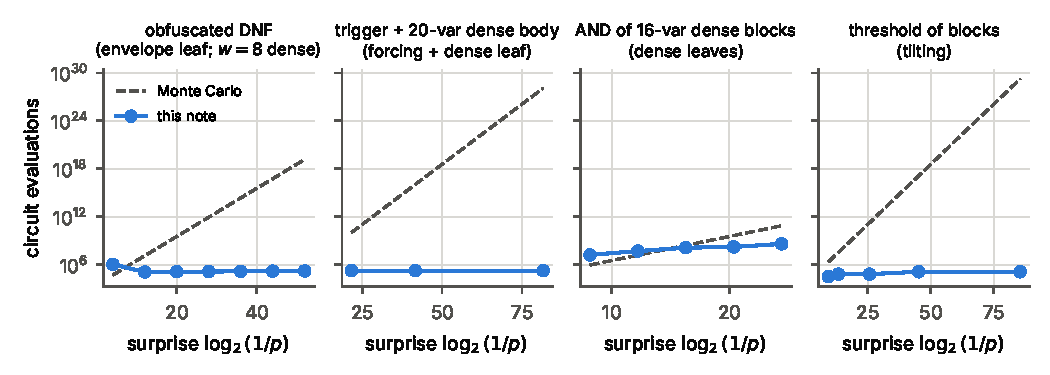
\includegraphics[width=\textwidth]{figures/fig_speedup.pdf}}{\fbox{figure pending}}
\caption{Circuit evaluations to reach an interval of ratio $\le1.1$ ($\eps=0.1$,
$\delta=0.05$) against the surprise $\log_2(1/p)$, compared with Monte Carlo's
requirement (\texttt{exp\_speedup.py}).}
\label{fig:speedup}
\end{figure}

\begin{table}[ht]
\centering\scriptsize
\begin{tabular}{llrrrrr}
\toprule
family & param & $p$ & interval ratio & cost & Monte Carlo & speed-up\\
\midrule
dnf-obfuscated & 8 & $6.08\cdot10^{-2}$ & 1.032 & $1.02\cdot10^{3}$ & $5.02\cdot10^{4}$ & $49.1$\\
dnf-obfuscated & 16 & $2.44\cdot10^{-4}$ & 1.073 & $6.55\cdot10^{4}$ & $1.33\cdot10^{7}$ & $2.03\cdot10^{2}$\\
dnf-obfuscated & 24 & $9.54\cdot10^{-7}$ & 1.083 & $1.00\cdot10^{6}$ & $3.41\cdot10^{9}$ & $3.41\cdot10^{3}$\\
dnf-obfuscated & 32 & $3.73\cdot10^{-9}$ & 1.808 & $1.00\cdot10^{6}$ & $8.73\cdot10^{11}$ & $8.73\cdot10^{5}$\\
dnf-obfuscated & 40 & $1.46\cdot10^{-11}$ & 270695.667 & $1.00\cdot10^{6}$ & $2.23\cdot10^{14}$ & $2.23\cdot10^{8}$\\
dnf-obfuscated & 48 & $5.68\cdot10^{-14}$ & inf & $1.00\cdot10^{6}$ & $5.72\cdot10^{16}$ & $5.72\cdot10^{10}$\\
trigger & 10 & $3.05\cdot10^{-4}$ & 1.087 & $1.02\cdot10^{3}$ & $1.06\cdot10^{7}$ & $1.04\cdot10^{4}$\\
trigger & 20 & $2.38\cdot10^{-7}$ & 1.004 & $1.02\cdot10^{3}$ & $1.36\cdot10^{10}$ & $1.33\cdot10^{7}$\\
trigger & 30 & $4.66\cdot10^{-10}$ & 1.091 & $4.10\cdot10^{3}$ & $6.98\cdot10^{12}$ & $1.70\cdot10^{9}$\\
trigger & 40 & $3.41\cdot10^{-13}$ & 1.087 & $2.05\cdot10^{3}$ & $9.53\cdot10^{15}$ & $4.65\cdot10^{12}$\\
trigger & 60 & $4.00\cdot10^{-19}$ & 1.066 & $1.45\cdot10^{5}$ & $8.13\cdot10^{21}$ & $5.61\cdot10^{16}$\\
trigger & 80 & $7.24\cdot10^{-25}$ & 1.029 & $1.92\cdot10^{4}$ & $4.49\cdot10^{27}$ & $2.34\cdot10^{23}$\\
blocks & 4 & $1.27\cdot10^{-2}$ & 1.082 & $8.19\cdot10^{3}$ & $2.53\cdot10^{5}$ & $30.9$\\
blocks & 8 & $1.85\cdot10^{-3}$ & 1.029 & $2.11\cdot10^{6}$ & $1.75\cdot10^{6}$ & $0.829$\\
blocks & 16 & $1.33\cdot10^{-5}$ & 1.066 & $5.88\cdot10^{6}$ & $2.45\cdot10^{8}$ & $41.7$\\
blocks & 24 & $3.86\cdot10^{-9}$ & 1.115 & $1.38\cdot10^{7}$ & $8.43\cdot10^{11}$ & $6.12\cdot10^{4}$\\
blocks & 32 & $3.62\cdot10^{-11}$ & 1.361 & $2.44\cdot10^{7}$ & $8.98\cdot10^{13}$ & $3.69\cdot10^{6}$\\
threshold & 50 & $5.59\cdot10^{-3}$ & 1.083 & $3.28\cdot10^{4}$ & $5.78\cdot10^{5}$ & $17.6$\\
threshold & 100 & $4.10\cdot10^{-5}$ & 1.087 & $3.28\cdot10^{4}$ & $7.92\cdot10^{7}$ & $2.42\cdot10^{3}$\\
threshold & 200 & $7.74\cdot10^{-8}$ & 1.089 & $6.55\cdot10^{4}$ & $4.20\cdot10^{10}$ & $6.41\cdot10^{5}$\\
threshold & 400 & $2.51\cdot10^{-15}$ & 1.079 & $1.31\cdot10^{5}$ & $1.29\cdot10^{18}$ & $9.87\cdot10^{12}$\\
threshold & 800 & $7.79\cdot10^{-27}$ & 1.096 & $3.28\cdot10^{4}$ & $4.17\cdot10^{29}$ & $1.27\cdot10^{25}$\\
\bottomrule
\end{tabular}

\caption{The runs of \cref{fig:speedup}. ``Cost'' counts all circuit evaluations,
including pilots and box estimation.}
\label{tab:speedup}
\end{table}

\paragraph{Context width (\cref{tab:ctx}).} ORs of $t$ CNFs with clauses on
sliding windows of width $w$, each CNF along its own random variable order, built as
left-deep $\wedge$-chains in window order (the bracketing of \cref{lem:pathcw}, kept by
the unflattened NNF). The compiler of \cref{thm:cw} finds context width $w$, the bound
of \cref{ex:or-cnf}, and produces an equivalent DNNF; the envelope estimator on it needs
only the minimum batch of $1{,}024$ samples, because the top $\vee$'s children are rare and almost
disjoint ($K\approx1$). Instances with $n\le24$ agree with enumeration.

\begin{table}[ht]
\centering\scriptsize
\IfFileExists{tables/ctx.tex}{\begin{tabular}{rrrrrrrrr}
\toprule
$n$ & $t$ & $w$ & cw & $|C|$ & DNNF size & interval for $p$ & samples & time (s)\\
\midrule
20 & 4 & 3 & 3 & 249 & 640 & [$0.39$, $0.416$] ($p=$0.393$$) & 1024 & 0.1\\
24 & 4 & 3 & 3 & 304 & 627 & [$0.209$, $0.221$] ($p=$0.215$$) & 1024 & 0.1\\
100 & 4 & 3 & 3 & 1375 & 2350 & [$9.50\cdot10^{-6}$, $9.54\cdot10^{-6}$] & 1024 & 0.6\\
200 & 4 & 3 & 3 & 2757 & 4575 & [$1.57\cdot10^{-11}$, $1.58\cdot10^{-11}$] & 1024 & 0.8\\
400 & 4 & 3 & 3 & 5633 & 8927 & [$2.91\cdot10^{-23}$, $2.92\cdot10^{-23}$] & 1024 & 2.1\\
800 & 8 & 3 & 3 & 22300 & 33927 & [$3.93\cdot10^{-46}$, $3.95\cdot10^{-46}$] & 1024 & 10.8\\
400 & 4 & 5 & 5 & 7115 & 15137 & [$1.46\cdot10^{-5}$, $1.46\cdot10^{-5}$] & 1024 & 6.0\\
\bottomrule
\end{tabular}
}{(table pending)}
\caption{Context-width compilation of ORs of window-CNFs (\texttt{exp\_ctx.py}).}
\label{tab:ctx}
\end{table}

\paragraph{Certified independence (\cref{tab:janson}).} Unate random $k$-CNFs with
up to $2\cdot10^5$ clauses: the Harris--Janson interval is deterministic, takes
seconds to a few minutes in Python, and on $200$ small instances it contained the exact
$p$ every time. At $n=2\cdot10^6$, $p\in[6.18,7.35]\cdot10^{-22}$; Monte Carlo would need
about $10^{24}$ evaluations for the same ratio. The second-order sandwich of
\cref{app:second-order} was checked against enumeration on 382 random instances with
no violations.

\begin{table}[ht]
\centering\scriptsize
\IfFileExists{tables/janson.tex}{\begin{tabular}{rrrrrr}
\toprule
$n$ & clauses & width & certified interval & ratio & time (s)\\
\midrule
10000 & 2000 & 10 & [$0.141$, $0.148$] & 1.039 & 0.8\\
100000 & 20000 & 12 & [$7.57\cdot10^{-3}$, $7.84\cdot10^{-3}$] & 1.035 & 11.0\\
200000 & 60000 & 12 & [$4.33\cdot10^{-7}$, $5.07\cdot10^{-7}$] & 1.167 & 50.3\\
1000000 & 200000 & 14 & [$4.99\cdot10^{-6}$, $5.15\cdot10^{-6}$] & 1.030 & 194.2\\
2000000 & 200000 & 12 & [$6.18\cdot10^{-22}$, $7.35\cdot10^{-22}$] & 1.187 & 71.0\\
\bottomrule
\end{tabular}
}{(table pending)}
\caption{Harris--Janson sandwich for random unate CNFs (\texttt{exp\_janson.py}).}
\label{tab:janson}
\end{table}

\paragraph{Certified telescoping (\cref{tab:cftp}).} Hard-core ladders: $x\sim
\mathrm{Bern}(0.3)^{n}$ and $C$ = ``$x$ is an independent set of the $2\times L$
ladder''. Janson's $\Delta$ is extensive, so the sandwich is useless; bounding-chain
CFTP gives exact samples, the truncation certificates contribute a bias factor below
$e^{0.02}$, and the certified intervals contain the exact $p$ (from variable
elimination).
In pure Python the constants are poor (each CFTP run costs thousands of updates), so
for these moderate $p$ Monte Carlo is still cheaper; the point is that the cost grows
polynomially in $L$ while $1/p$ grows exponentially, and that the method is sound
without any mixing-time proof.

\begin{table}[ht]
\centering\scriptsize
\IfFileExists{tables/cftp.tex}{\begin{tabular}{rrrlll}
\toprule
$L$ & $n$ & $p$ (exact) & Harris--Janson window & certified telescoping & CFTP runs\\
\midrule
20 & 40 & $2.31\cdot10^{-2}$ & [$4.21\cdot10^{-3}$, $0.107$] & [$2.07\cdot10^{-2}$, $2.69\cdot10^{-2}$] & $2.34\cdot10^{5}$\\
40 & 80 & $4.90\cdot10^{-4}$ & [$1.46\cdot10^{-5}$, $1.18\cdot10^{-2}$] & [$4.15\cdot10^{-4}$, $6.06\cdot10^{-4}$] & $4.42\cdot10^{5}$\\
60 & 120 & $1.04\cdot10^{-5}$ & [$5.12\cdot10^{-8}$, $1.31\cdot10^{-3}$] & [$8.36\cdot10^{-6}$, $1.35\cdot10^{-5}$] & $6.76\cdot10^{5}$\\
\bottomrule
\end{tabular}
}{(table pending)}
\caption{Certified telescoping on hard-core ladders (\texttt{exp\_cftp.py}).}
\label{tab:cftp}
\end{table}

\paragraph{Local thresholds (\cref{tab:local}).} \Cref{sec:local} reports the tilted
Glauber estimator on chain and random-cubic-graph local threshold circuits with random
local tables ($p$ down to $10^{-23.7}$ with certified Glauber samplers, and
$10^{-169.8}$ with coupling from the past beyond the Dobrushin regime), checked against
exact transfer-matrix values for chains and $10^7$ Monte Carlo samples for a small
cubic instance (\texttt{exp\_local.py}).

\paragraph{Affine structure (\cref{tab:affine}).} \Cref{sec:affine} reports the
presolve, affine envelopes, XPT arguments and DFSB on parity-check families under
uniform and biased product distributions, with exact values computed without the
module under test (\texttt{exp\_affine.py}).

\paragraph{What the prover adds (\cref{tab:arguments}, \cref{fig:proofs}).}
Hidden triggers $R\wedge T(x_S)$ whose test accepts only $x_S=a$:
\emph{linear-hash} tests $[Mx_S=Ma]$ with a dense $(k+4)\times k$ matrix over
$\F_2$, and \emph{SPN} tests $[\mathrm{SPN}(x_S)=\mathrm{SPN}(a)]$ with random
bijective 4-bit S-boxes and dense invertible linear layers. Without a prover,
Gaussian-elimination forcing recognises linear hashes. SPN tests are reached only
through small-cone canonicalisation: a test on at most $a=12$ variables is an atom
whose OBDD exposes $x_S=a$ to forcing, and DFSB reduces larger tests to atoms by
branching, with about $2^{|S|-a}$ leaves. With a prover, the argument is the subcube
$x_S=a$ plus a DRUP proof (from Glucose) that $C\Rightarrow(x_S=a)$; the verifier
checks it with its own RUP checker and samples only $R$. The DRUP proofs found by the
solver grow exponentially with $k$ even for linear hashes (CDCL solvers do not perform
Gaussian elimination); this is evidence, not a resolution lower bound, that the class
of \cref{thm:certenv} depends on the proof system.

\begin{table}[ht]
\centering\scriptsize
\IfFileExists{tables/arguments.tex}{\begin{tabular}{lrrrrrrr}
\toprule
family & $k$ & $|C|$ & $p$ & Part 1 ratio & proof steps & check (s) & Part 2 ratio\\
\midrule
linear hash & 12 & 78 & $1.53\cdot10^{-4}$ & 1 & 329 & 0.0 & 1.088\\
linear hash & 16 & 86 & $3.81\cdot10^{-6}$ & 1 & 1269 & 0.2 & 1.079\\
linear hash & 20 & 82 & $5.96\cdot10^{-7}$ & 1 & 5717 & 2.1 & 1.093\\
linear hash & 24 & 96 & $2.98\cdot10^{-8}$ & 1 & 32910 & 81.4 & 1.085\\
SPN, 2 rounds & 8 & 246 & $3.85\cdot10^{-3}$ & 1 & 278 & 0.0 & 1.027\\
SPN, 2 rounds & 12 & 334 & $1.37\cdot10^{-4}$ & 1 & 697 & 0.2 & 1.074\\
SPN, 3 rounds & 16 & 609 & $6.68\cdot10^{-6}$ & 1 & \multicolumn{3}{l}{no proof within 1200 s}\\
SPN, 3 rounds & 20 & 756 & $9.54\cdot10^{-7}$ & none in 900 s & 25944 & 39.5 & 1.004\\
\bottomrule
\end{tabular}
}{(table pending)}
\caption{Hidden triggers with and without a prover (\texttt{exp\_arguments.py}).
Part 1 ratio is that of the DFSB interval ($\infty$: lower end $0$); Part 2 ratio
is that of the verifier's interval after checking the proof.}
\label{tab:arguments}
\end{table}

\begin{figure}[ht]
\centering
\begin{minipage}{0.48\textwidth}\centering
\IfFileExists{figures/fig_proofs.pdf}{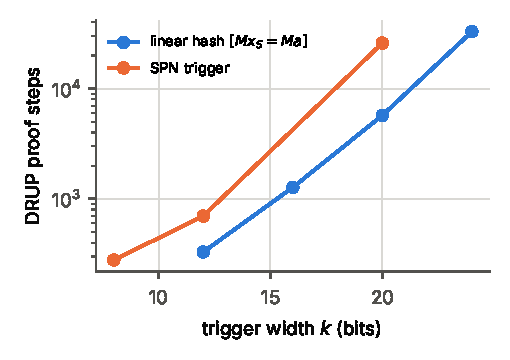
\includegraphics[width=\textwidth]{figures/fig_proofs.pdf}}{\fbox{figure pending}}
\caption{DRUP proof size for hidden triggers.}\label{fig:proofs}
\end{minipage}\hfill
\begin{minipage}{0.48\textwidth}\centering
\IfFileExists{figures/fig_surprise.pdf}{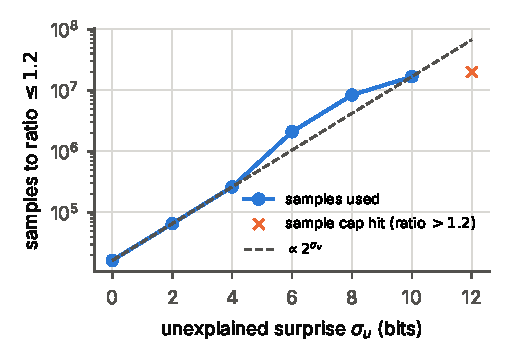
\includegraphics[width=\textwidth]{figures/fig_surprise.pdf}}{\fbox{figure pending}}
\caption{Surprise accounting: samples needed when an argument reveals all but
$\sigma_u$ bits of a 40-bit trigger.}\label{fig:surprise}
\end{minipage}
\end{figure}

\paragraph{Surprise accounting (\cref{fig:surprise}).} For a 40-bit trigger, an
argument that reveals $40-\sigma_u$ of the bits (a subcube envelope on those bits)
leaves $\sigma_u$ bits to sampling; the number of samples grows as $2^{\sigma_u}$, as
\cref{thm:surprise} says it must.

\section{Discussion and open problems}\label{sec:discussion}

\paragraph{What the answers are.}
Without a prover, one can beat sampling exactly where the rarity of $C(x)=1$
is \emph{visible}: built from independent parts, forced literals, small
cutsets, unions, thresholds of independent blocks, or sparse monotone
overlaps, possibly disguised by local rewriting. DFSB plus the specialised
modules is sound on every circuit and costs $\poly\cdot K$ on the circuits whose
ideal $K$-explanation tree is small (\cref{thm:dfsb,thm:meta}). With a prover,
the visible structure may be replaced by \emph{provable} structure: anything a
propositional proof system can certify about where the rare inputs live
(\cref{thm:certenv}). In both settings the cost has the same shape, polynomial
in the explained surprise and exponential in the unexplained surprise, and the
exponential part is unavoidable for black-box residuals (\cref{thm:surprise}).

\paragraph{Relation to heuristic arguments.}
ARC's programme \cite{christiano2022presumption,hilton2024surprise} asks for
estimators that use a model's internals to beat sampling, and measures
explanations by surprise accounting. The present results isolate the part of
that programme that can be made \emph{sound against adversarial circuits}:
\begin{itemize}
\item the presumption of independence is certified where independence is
syntactic (variable-disjoint parts, \textsc{prod}) or where correlation
inequalities control the error (\cref{thm:janson});
\item surprise accounting becomes a cost formula for a sound verifier,
$\poly(|\pi|)+2^{\sigma_u(\pi)}$ up to polynomial factors, and both halves have
black-box lower bounds: a bit of argument saves at most a factor $2$ in
evaluations for lower bounds, and the $2^{\sigma_u}$ term is unavoidable for
two-sided intervals once the envelope is fixed (\cref{thm:surprise});
\item what soundness forbids is equally sharp: upper bounds must come from
deduction (\cref{thm:blackbox}), and no system certifies them for all circuits
(\cref{thm:ma}). A heuristic estimator that is accurate on random circuits but
not sound on adversarial ones is therefore not a counterexample to anything
here; it lives in the gap between ``no certificate exists'' and ``the estimate
is wrong''.
\end{itemize}
The rarity that defeats certification is \emph{distributed surprise}: many
weak, overlapping constraints (random CNFs below the threshold), or
pseudorandomness. Annealing and splitting estimators handle the first in
practice, and ARC-style heuristic estimators may handle both on typical
instances; neither comes with a certificate that a polynomial-time verifier can
check.

\paragraph{Open problems.}
\begin{enumerate}
\item \emph{Envelope lower bounds for distributed surprise.} Does every
polynomial-size DNNF envelope of a random 3-CNF with $1/3<\alpha<\alpha_{\rm sat}$
have $D(E)/p=2^{\Omega(n)}$? Proved here only for drop-conjunct relaxations.
\item \emph{Certified annealing.} Is there any polynomial-size, MA-checkable
certificate that a sampler for $D\mid A_1\wedge\dots\wedge A_j$ is accurate (a
checkable mixing certificate)? By \cref{thm:blackbox} it cannot be purely
statistical. This is what would make multilevel splitting sound.
\item \emph{Nested unions over approximate leaves.} Can the DNNF FPRAS be run
over DNNF skeletons whose leaves are sets given only by approximate counters,
approximate samplers and membership tests? This would give unions of unions of
products of dense blocks at any depth.
\item \emph{A natural two-sided separation.} Find a $\mathsf{UP}\cap\mathsf{coUP}$
problem not in $\BPP$ (under a standard assumption) whose unique-witness property
has polynomial-size extended Frege proofs; then the two-sided separation holds
with a standard proof checker instead of a theory like ZFC.
\item \emph{Optimal arguments.} How well can $\min_\pi\big(|\pi|+2^{\sigma_u(\pi)}\big)$
be approximated for natural certificate languages? Choosing which conjuncts to
keep is weighted set packing on supports; choosing branch variables is related to
pseudo-tree depth.
\item \emph{Networks.} Binarised or ReLU networks with rare activation patterns
are the case of most interest for alignment. Interval-bound propagation already
gives gate-wise outer approximations; can it be turned into sandwich certificates
(\cref{sec:part2}) with small looseness for trained networks?
\item \emph{Heuristic to certified.} When a presumption-of-independence estimate
is accurate, when can it be compiled into a certificate with polynomial overhead,
for instance by proving the independence it presumes, or by bounding the
correlations it ignores?
\end{enumerate}

\appendix

\section{The second-order independence sandwich}\label{app:second-order}

Setting of \cref{thm:janson-general}: increasing events $B_1,\dots,B_m$ (after
flipping the variables that occur positively, \cref{sec:independence}) with syntactic
supports $S_i$, a product distribution, and a fixed order. For each $i$ let
$N_i=\{j<i:j\sim i\}$, $R_i=\{j<i:j\not\sim i\}$, $\Gamma(j)$ the neighbourhood of $j$,
$b_i=D(B_i)$ with $\max_ib_i<1$, $\beta_i=\sum_{j\in N_i}b_j$ (assumed $<1$),
\[
C_i=\sum_{j\in N_i}\mathrm{Cov}(B_i,B_j)\ \ (\ge0\text{ by Harris}),
\]
\[
\Theta_i=b_i\Big[\sum_{j\in N_i}\sum_{k\in R_i\cap\Gamma(j)}D(B_jB_k)+\sum_{j<j'\in N_i}D(B_jB_{j'})\Big],
\]
\[
\Theta'_i=\sum_{j\in N_i}\sum_{k\in R_i\cap\Gamma(j)}D(B_iB_jB_k)+\sum_{j<j'\in N_i}D(B_iB_jB_{j'}).
\]
Each triple $\{i,j,k\}$ with $j,k<i$ that is connected in $G$ occurs exactly once in
these sums (in the first if $i$ is adjacent to only one of $j,k$, in the second if it
is adjacent to both), so $\Theta'_i=\sum D(B_iB_jB_k)$ and $\Theta_i=b_i\sum D(B_jB_k)$
over these triples, and $\sum_i\Theta'_i$ does not depend on the order. If $b_i=0$
then $c_i$, $C_i$, $\Theta_i$ and $\Theta'_i$ vanish and the $i$-th factors below equal $1$;
so we assume $b_i>0$ whenever we condition on $B_i$.

\begin{theorem}\label{thm:second-order}
\[
\prod_i\Big(1-\min\Big\{b_i,\;b_i-C_i+\frac{\Theta'_i}{1-\beta_i}\Big\}\Big)\;\le\;p\;\le\;
\prod_i\Big(1-\max\Big\{0,\;b_i-\frac{C_i+\Theta_i}{1-\beta_i}\Big\}\Big).
\]
Consequently, with $M_2=\prod_i(1-b_i+C_i)$,
$|\log p-\log M_2|\le E_3:=\sum_i\frac{\Theta_i+\Theta'_i+\beta_iC_i}{(1-\beta_i)(1-b_i)}$.
\end{theorem}

\begin{proof}
Fix $i$, write $N=N_i$, $R=R_i$, $F_X=\bigwedge_{j\in X}\neg B_j$ and
$\nu=D(\cdot\mid F_R)$ (by Harris $\Pr[F_R]\ge\prod_{j\in R}(1-b_j)>0$). Then $p=\prod_i(1-c_i)$ with $c_i=\Pr[B_i\mid F_N\wedge F_R]$.
Since $S_i$ is disjoint from the supports of the events in $R$, $\nu(B_i)=b_i$ and
\[
c_i=b_i-\frac{b_i\,[\nu(F_N)-\nu(F_N\mid B_i)]}{\nu(F_N)},\qquad
\nu(F_N)-\nu(F_N\mid B_i)=\nu\big(\textstyle\bigcup_NB_j\mid B_i\big)-\nu\big(\textstyle\bigcup_NB_j\big).
\]
We use six facts. Each follows from the Harris inequality (an increasing and a
decreasing event are negatively correlated under a product measure) and from
independence of events with disjoint supports. For $j\in N$ let $R'=R\cap\Gamma(j)$
and $R''=R\setminus R'$; the events of $R''$ have supports disjoint from
$S_i\cup S_j$, and $\Pr[F_R]\le\Pr[F_{R''}]$.
\begin{enumerate}[label=(H\arabic*)]
\item $\nu(B_j\mid B_i)\le D(B_iB_j)/b_i$ (Harris for $B_iB_j$ versus $F_R$).
\item $\nu(B_j)\le b_j$ (Harris).
\item $\nu(B_j)\ge b_j-\sum_{k\in R'}D(B_jB_k)$: $\Pr[B_jF_R]\ge\Pr[B_jF_{R''}]-\sum_{k\in
R'}\Pr[B_jB_kF_{R''}]\ge(b_j-\sum_kD(B_jB_k))\Pr[F_{R''}]$ by independence and Harris;
divide by $\Pr[F_R]\le\Pr[F_{R''}]$ (trivial if the bracket is negative).
\item $\nu(B_jB_{j'})\le D(B_jB_{j'})$ (Harris).
\item $\nu(B_j\mid B_i)\ge\big[D(B_iB_j)-\sum_{k\in R'}D(B_iB_jB_k)\big]/b_i$: as (H3), with
$B_iB_j$ in place of $B_j$.
\item $\nu(B_jB_{j'}\mid B_i)\le D(B_iB_jB_{j'})/b_i$ (Harris).
\end{enumerate}
\emph{Upper bound on $p$.} By Bonferroni, $\nu(\bigcup B_j\mid B_i)\le\sum_j\nu(B_j\mid
B_i)$ and $\nu(\bigcup B_j)\ge\sum_j\nu(B_j)-\sum_{j<j'}\nu(B_jB_{j'})$. With (H1), (H3),
(H4), $b_i[\nu(F_N)-\nu(F_N\mid B_i)]\le C_i+\Theta_i$; with (H2), $\nu(F_N)\ge1-\beta_i$.
So $c_i\ge b_i-(C_i+\Theta_i)/(1-\beta_i)$, and $c_i\ge0$.

\emph{Lower bound on $p$.} By Bonferroni the other way with (H5), (H6), (H2),
$b_i[\nu(F_N)-\nu(F_N\mid B_i)]\ge C_i-\Theta'_i$. If $C_i\ge\Theta'_i$ use
$\nu(F_N)\le1$; otherwise use $\nu(F_N)\ge1-\beta_i$. In both cases (using $C_i\ge0$)
$c_i\le b_i-C_i+\Theta'_i/(1-\beta_i)$; and $c_i\le b_i$ by Harris.

\emph{The $E_3$ bound.} Put $x_i=1-b_i+C_i\ge1-b_i$. On the upper side, the factor is
at most $x_i+(\Theta_i+\beta_iC_i)/(1-\beta_i)$ (or $1$, in which case
$1-x_i<(\Theta_i+\beta_iC_i)/(1-\beta_i)$), and $\log(x+y)-\log x\le y/x$. On the lower
side, the factor is at least $\max\{1-b_i,\ x_i-\Theta'_i/(1-\beta_i)\}$; if the
second term is the larger one, $\log(x-y)-\log x\ge-y/(x-y)\ge-y/(1-b_i)$, and
otherwise $C_i<\Theta'_i/(1-\beta_i)$ and $\log(1-b_i)-\log x_i\ge-C_i/(1-b_i)$, which is
no smaller. Summing over $i$ gives the claim.
\end{proof}

We checked the theorem against exact enumeration on 382 random instances (3--8
random monotone events, each a monotone DNF on 2--4 of 8--14 variables, random product
distributions and orders; \texttt{experiments/check\_second\_order.py}): no
violations, median $E_3=0.064$. The $\min$ in the lower bound matters: without it a
factor can become negative, and a product of two negative factors can exceed $p$.


\bibliographystyle{alpha}
\bibliography{refs}

\end{document}
